\documentclass[12pt]{article}
% \usepackage[top=1in,left=1in, right = 1in, footskip=1in]{geometry}
\usepackage[top=1in,footskip=1in]{geometry}

\usepackage{graphicx}
\usepackage{xspace}
%\usepackage{adjustbox}

\usepackage{pdflscape}

\usepackage{grffile}

\newcommand{\comment}{\showcomment}
%% \newcommand{\comment}{\nocomment}

\newcommand{\showcomment}[3]{\textcolor{#1}{\textbf{[#2: }\textsl{#3}\textbf{]}}}
\newcommand{\nocomment}[3]{}

\newcommand{\swp}[1]{\comment{magenta}{SWP}{#1}}

\newcommand{\eref}[1]{Eq.~(\ref{eq:#1})}
\newcommand{\fref}[1]{Fig.~\ref{fig:#1}}
\newcommand{\Fref}[1]{Fig.~\ref{fig:#1}}
\newcommand{\sref}[1]{Sec.~\ref{#1}}
\newcommand{\frange}[2]{Fig.~\ref{fig:#1}--\ref{fig:#2}}
\newcommand{\tref}[1]{Table~\ref{tab:#1}}
\newcommand{\tlab}[1]{\label{tab:#1}}
\newcommand{\seminar}{SE\mbox{$^m$}I\mbox{$^n$}R}

\usepackage{amsthm}
\usepackage{amsmath}
\usepackage{amssymb}
\usepackage{amsfonts}
\usepackage[utf8]{inputenc} % make sure fancy dashes etc. don't get dropped
\allowdisplaybreaks

\usepackage{lineno}
\linenumbers

\usepackage[pdfencoding=auto, psdextra]{hyperref}

\usepackage{natbib}
\bibliographystyle{unsrt}
\date{\today}

\usepackage{xspace}
\newcommand*{\ie}{i.e.\@\xspace}

\usepackage{color}

\newcommand{\Rx}[1]{\ensuremath{{\mathcal R}_{#1}}\xspace} 
\newcommand{\RR}{\ensuremath{{\mathcal R}}\xspace}
\newcommand{\Rres}{\Rx{\mathrm{res}}}
\newcommand{\Rinv}{\Rx{\mathrm{inv}}}
\newcommand{\Rhat}{\ensuremath{{\hat\RR}}}
\newcommand{\Rt}{\ensuremath{{\mathcal R}(t)}\xspace}
\newcommand{\tsub}[2]{#1_{{\textrm{\tiny #2}}}}
\newcommand{\dd}[1]{\ensuremath{\, \mathrm{d}#1}}
\newcommand{\dtau}{\dd{\tau}}
\newcommand{\dx}{\dd{x}}
\newcommand{\dsigma}{\dd{\sigma}}

\newcommand{\rx}[1]{\ensuremath{{r}_{#1}}\xspace} 
\newcommand{\rres}{\rx{\mathrm{res}}}
\newcommand{\rinv}{\rx{\mathrm{inv}}}

\newcommand{\psymp}{\ensuremath{p}} %% primary symptom time
\newcommand{\ssymp}{\ensuremath{s}} %% secondary symptom time
\newcommand{\pinf}{\ensuremath{\alpha_1}} %% primary infection time
\newcommand{\sinf}{\ensuremath{\alpha_2}} %% secondary infection time

\newcommand{\psize}{{\mathcal P}} %% primary cohort size
\newcommand{\ssize}{{\mathcal S}} %% secondary cohort size

\newcommand{\gtime}{\tau_{\rm g}} %% generation interval
\newcommand{\gdist}{g} %% generation-interval distribution
\newcommand{\idist}{\ell} %% incubation-period distribution

\newcommand{\total}{{\mathcal T}} %% total number of serial intervals

\usepackage{lettrine}

\newcommand{\dropcapfont}{\fontfamily{lmss}\bfseries\fontsize{26pt}{28pt}\selectfont}
\newcommand{\dropcap}[1]{\lettrine[lines=2,lraise=0.05,findent=0.1em, nindent=0em]{{\dropcapfont{#1}}}{}}

\begin{document}

\begin{flushleft}{
	\Large
	\textbf\newline{
		Susceptible host dynamics explain pathogen resilience to perturbations
	}
}
\newline
\\
Sang Woo Park, \dots, Bryan T. Grenfell, Sarah Cobey
\\
\bigskip
\end{flushleft}

\section*{Abstract}

Major priority for epidemiological research in the time of anthropogenic change is understanding how infectious disease dynamics respond to perturbations.
Interventions to slow the spread of SARS-CoV-2 significantly disrupted the transmission of other human pathogens. 
As interventions lifted, whether and when respiratory pathogens would eventually return to their pre-pandemic dynamics remains to be answered. 
We develop a framework for estimating pathogen resilience based on how fast epidemic patterns return to their pre-pandemic, endemic dynamics.
Our analysis suggests that some pathogens may have settled to endemic cycles that are different from their pre-pandemic patterns.
Finally, we show that the replenishment rate of the susceptible pool is a key determinant of pathogen resilience.
Our framework offers a novel perspective to characterizing the dynamics of endemic pathogens and their responses to SARS-CoV-2 interventions.
\swp{Need to emphasize broader implications.}

\pagebreak

Non-pharmaceutical interventions (NPIs) to slow the spread of SARS-CoV-2 disrupted the transmission of other human respiratory pathogens, adding uncertainties to their future epidemic dynamics and the overall public health burden \citep{baker2020impact}.
As NPIs lifted, large heterogeneities in outbreak dynamics were observed across different pathogens in different countries, with some pathogens exhibiting earlier resurgences than others \citep{gomez2021uncertain,koltai2022determinants,park2024predicting}.
Heterogeneities in the overall reduction in transmission and the timing of re-emergence likely reflect differences in NPI patterns, pathogen characteristics, immigration/importation from other countries, and pre-pandemic pathogen dynamics \citep{perofsky2024impacts}.
Therefore, comparing the differential impact of the pandemic perturbations across pathogens can provide unique opportunities to learn about underlying pathogen characteristics, such as their transmissibility or duration of immunity, from heterogeneities in re-emergence patterns \citep{chow2023effects}.

\begin{figure}[!th]
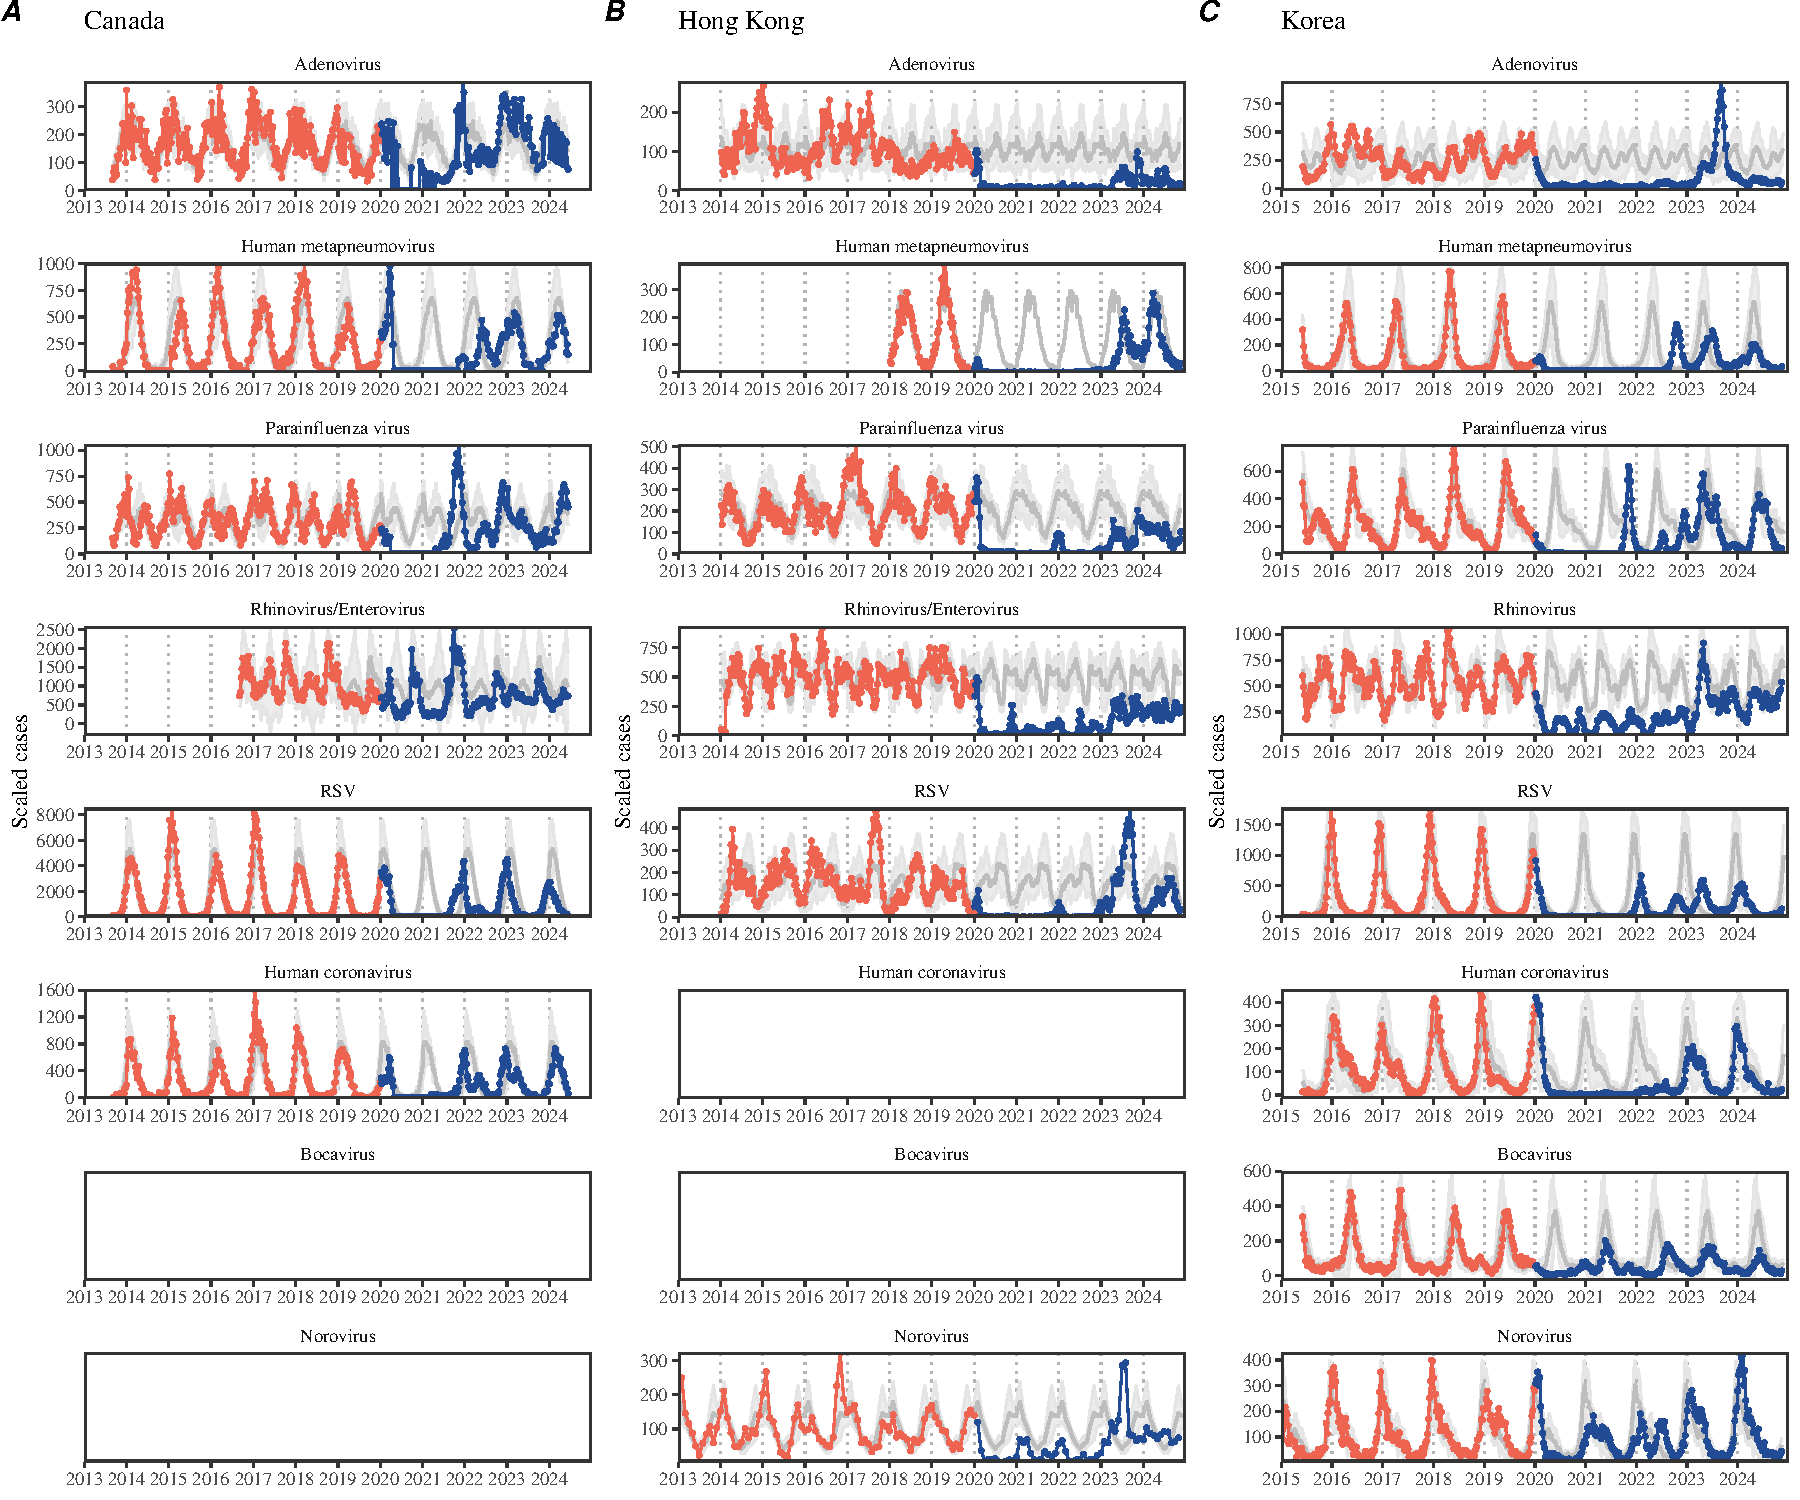
\includegraphics[width=\textwidth]{../figure1/figure1.pdf}
\caption{
\textbf{Observed heterogeneity in responses to pandemic perturbations across respiratory pathogens and norovirus in (A) Canada, (B) Hong Kong, (C) Korea, and (D) US.}
Red points and lines represent data before 2020.
Blue points and lines represent data since 2020.
Gray lines and shaded regions represent the mean seasonal patterns and corresponding 95\% confidence intervals around the mean.
Mean seasonal patterns were calculated by aggregating cases before 2020 into 52 weekly bins and taking the average in each week.
Cases were scaled to account for changes in testing patterns (Materials and Methods).
}
\end{figure} 

Even though more than five years have passed since the emergence of SARS-CoV-2, we still observe persistent changes in pathogen dynamics following the pandemic perturbations: 
for example, compared to pre-pandemic, seasonal patterns, human metapneumovirus in Korea seem to circulate at lower levels, whereas RSV in Korea seem to exhibit different seasonality (Figure 1).
These observations suggest a possibility for a fundamental change in pathogen dynamics following the pandemic perturbations, which can be driven by permanent shift in either human behavior or population-level immunity \citep{kissler2020projecting,baker2022long}.
The possibility of a long-lasting impact of the pandemic perturbations pose an important question for future infectious disease dynamics: can we predict whether and when other respiratory pathogens will eventually return to their pre-pandemic dynamics?
\swp{You suggested: I would say something about the dynamics of these pathogens not being well understood, but I've since rewritten the most of intro and I'm not sure where I would fit this. If you have any suggestions, let me know...}

So far, the majority of epidemiological analyses of respiratory pathogens in the context of the pandemic perturbations have focused on characterizing the timing of rebound \citep{baker2020impact,eden2022off,perofsky2024impacts}.
Instead, we seek to characterize how fast a pathogen returns to its pre-pandemic dynamics.
These two concepts have subtle but important differences: 
for example, it took more than 3 years for human metapneumovirus to rebound in Hong Kong but the observed epidemic patterns in 2024 are similar to pre-pandemic seasonal means, suggesting a rapid return to pre-pandemic dynamics following a perturbation (Figure 1).
Measuring this rate of return is particularly useful because it allows us to quantify the ecological resilience of a host-pathogen system \citep{pimm1979structure, neubert1997alternatives,gunderson2000ecological,dakos2022ecological}.

In this study, we lay out theoretical and statistical approaches to characterizing the resilience of a host-pathogen system based on how fast the system recovers from perturbation.
We begin by laying out a few representative scenarios that capture the potential impact of pandemic perturbations on endemic pathogen dynamics and illustrate how resilience can be measured by comparing the pre- and post-pandemic dynamics of susceptible and infected hosts.
In practice, information on susceptible hosts is often unavailable, making this theoretical approach infeasible.
Instead, we utilize a mathematical technique to reconstruct empirical attractors from the data \citep{takens2006detecting}, which allows us to measure the rate at which the host-pathogen system approaches this empirical attractor after a perturbation;
this rate corresponds to the resilience of the host-pathogen system.
We use this method to analyze pathogen surveillance data for respiratory and non-respiratory pathogens from Canada, Hong Kong, Korea, and US.
Finally, we show that susceptible host dynamics explain variation in pathogen resilience.
% Our study offers unique insights into understanding pathogen re-emergence patterns following COVID-19 interventions.
% \swp{Revisit.}
 
\section*{Conceptual introduction to pathogen resilience}

In classical ecological literature, resilience of an ecological system is measured by the rate at which the system returns to its reference state following a perturbation \citep{pimm1979structure, neubert1997alternatives,gunderson2000ecological,dakos2022ecological}.
This rate corresponds to the largest real part of the eigenvalues of the linearized system near equilibrium---here, we refer to this value as the \emph{intrinsic} resilience of the system, which represents the expected rate of return from perturbed states.
In practice, we rarely know the true model describing population-level dynamics of common respiratory pathogens, limiting our ability to infer the intrinsic resilience of a system.
Instead, we can still measure the \emph{empirical} resilience of a host-pathogen system by looking at how fast the system returns to the pre-pandemic, endemic dynamics after interventions are lifted.

As an example, we begin with a simple Susceptible-Infected-Recovered-Susceptible (SIRS) model with seasonally forced transmission and demography (i.e., birth and death).
The SIRS model is the simplest model that allows for waning of immunity and is commonly used for modeling the dynamics of respiratory pathogens \citep{dushoff2004dynamical}.
First, consider an intervention that reduce transmission by 50\% for 6 months starting in 2020, which causes epidemic patterns to deviate from its original stable annual cycle for a short period of time and eventually come back (Figure 2A).
To measure the resilience of this system empirically, we first need to be able to measure the distance from its pre-pandemic attractor.
There are many ways we can measure the distance from the attractor, but for illustrative purposes, we choose one of the most parsimonious approach: that is, we look at how the susceptible (S) and infected (I) populations change over time and measure the distance on the SI phase plane (Figure 2B).
In this simple case, the locally estimated scatterplot smoothing (LOESS) fit indicates that the distance from the attractor decreases exponentially (linearly on a log scale) on average (Figure 2C).
Furthermore, the overall rate of return approximates the intrinsic resilience of the seasonally unforced system (Figure 2C).

\begin{figure}[!th]
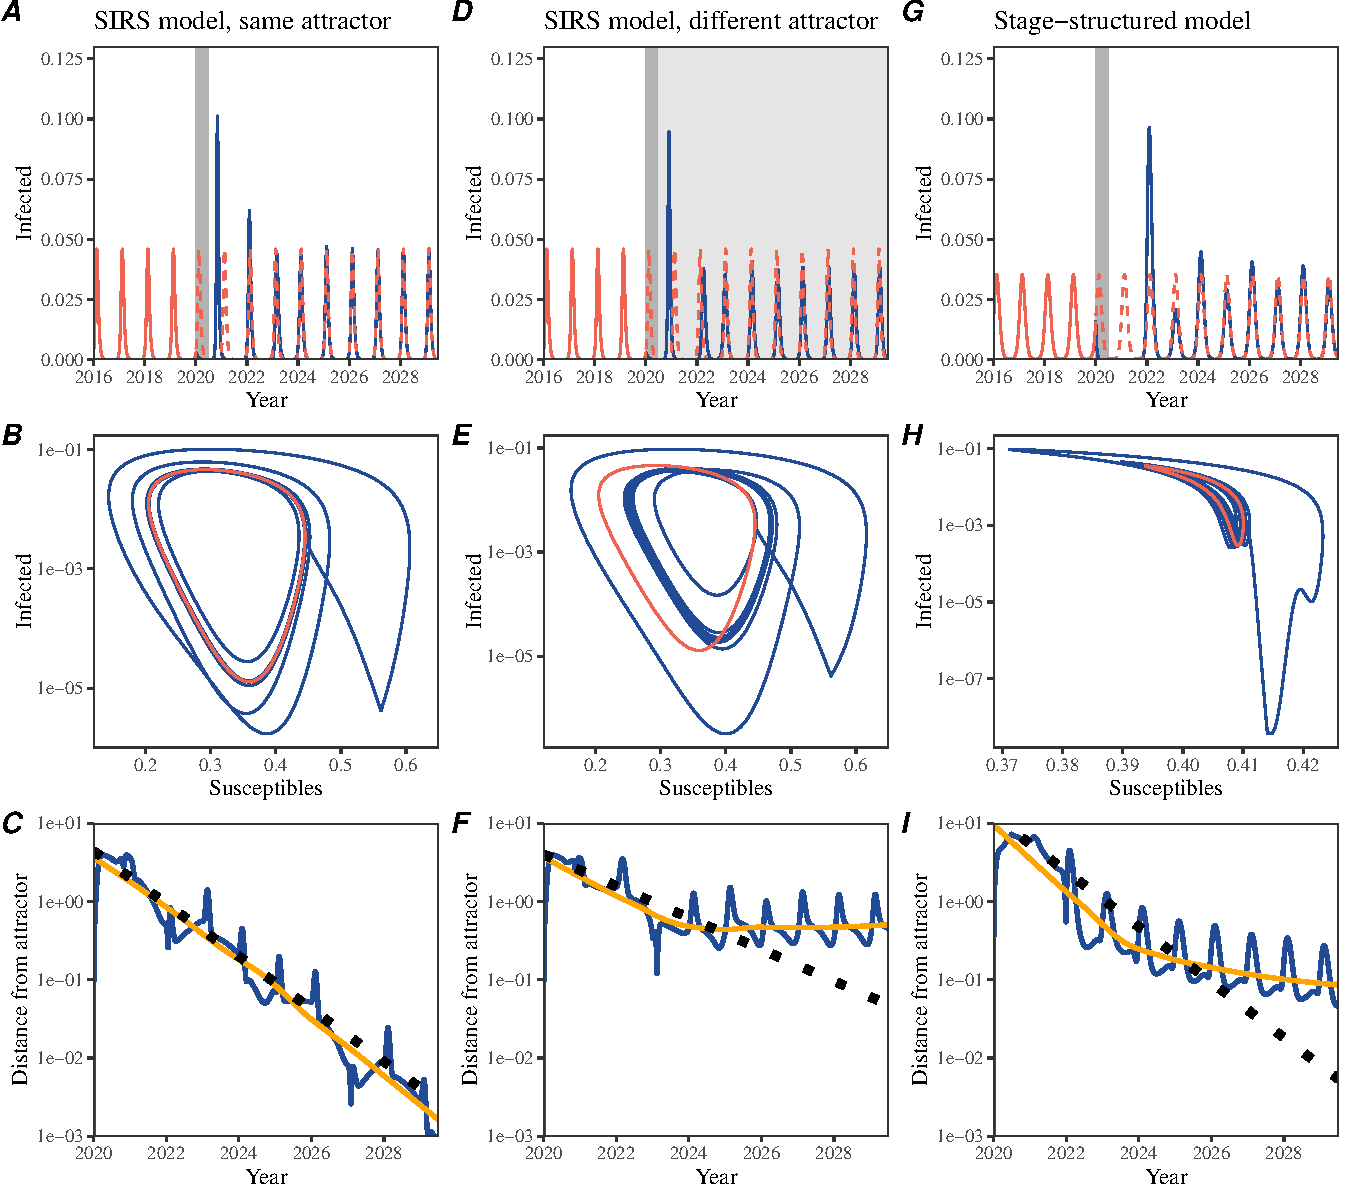
\includegraphics[width=\textwidth]{../figure2/figure2_simple.pdf}
\caption{
\textbf{A simple method to measure pathogen resilience following pandemic perturbations across different scenarios.}
(A, D, G) Simulated epidemic trajectories across various models. 
Red and blue solid lines represent epidemic dynamics before and after interventions are introduced, respectively.
Red dashed lines represent counterfactual epidemic dynamics in the absence of interventions.
Gray regions indicate the duration of interventions.
(B, E, H) Phase plane representation of the time series in panels A, D, and G alongside the corresponding susceptible host dynamics.
Red and blue solid lines represent epidemic trajectories on an SI phase plane before and after interventions are introduced, respectively.
(C, F, I) Changes in logged distance from the attractor over time.
Blue lines represent the logged distance from the attractor.
Orange lines represent the locally estimated scatterplot smoothing (LOESS) fits to the logged distance from the attractor.
Dotted lines show the intrinsic resilience of the seasonally unforced system.
}
\end{figure}

Alternatively, pandemic perturbations can have a lasting impact on the pathogen dynamics; 
as an example, we consider a scenario in which a 10\% reduction in transmission persists even after interevntions are lifted (Figure 2D--F).
In such cases in practice, we cannot know whether the pathogen will return to its original cycle or a different cycle until many years have passed, and we cannot measure the distance to the new unknown attractor that the system might eventually approach.
Nonetheless, we can still measure the distance from the pre-pandemic attractor and ask how the distance changes over time (Figure 2E).
The LOESS fit suggests that the distance from the pre-pandemic attractor will initially decrease exponentially on average (equivalently, linearly on a log scale) and eventually plateau (Figure 2F).
Here, a permanent 10\% reduction in transmission rate slows the system, which causes the distance from the pre-pandemic attractor initially to decrease at a slower rate (Figure 2F) than it would have otherwise (Figure 2C) before plateauing at a fixed distance between the two attractors.
This example shows that resilience is not necessarily an intrinsic property of a specific pathogen.
Instead, pathogen resilience is a property of a specific attractor that a host-pathogen system approaches, which depends on both pathogen and host characteristics.
% \swp{Add discussion about observation error, e.g., under-reporting.}

Finally, transient phenomena can further complicate the picture (Figure 2G--I).
For example, a stage-structured model initially exhibits a stable annual cycle, but perturbations from a 10\% reduction in transmission for 6 months cause the epidemic to shift to biennial cycles (Figure 2G).
The system eventually approaches the original pre-pandemic attractor (Figure 2H), suggesting that this biennial cycle is a transient phenomenon.
The LOESS fit indicates that the distance from the attractor initially decreases exponentially at a rate that is consistent with the intrinsic resilience of the seasonally unforced stage-structured system, but the rate of decrease decelerates with the damped oscillations (Figure 2I).
This behavior is also referred to as a ghost attractor, which causes long transient dynamics and slow transitions \citep{hastings2018transient}.
Strong seasonal forcing in transmission can also lead to transient phenomena for a simple SIRS model, causing a slow return to pre-perturbation dynamics (Supplementary Figure S1).

This empirical approach allows us to measure the resilience of a two-strain host-pathogen system even when we have incomplete observation of the infection dynamics.
Simulations from a simple two-strain system illustrate that separate analyses of individual strain dynamics (e.g., RSV A vs B) and a joint analysis of total infections (e.g., total RSV infections) yield identical resilience estimates (Supplementary Figure S2, 3).
This is expected because the dynamics of two strains (or two pathogens) around the attractor in a coupled system are described by the same set of eigenvalues and eigenvectors, meaning that both strains should exhibit identical rates of returns following a perturbation.
Analogous to a single system, strong seasonal forcing in transmission can cause the system to slow down through transient phenomena (Supplementary Figure S4).

These observations indicate three possibilities.
First, we can directly estimate the empirical resilience of a host-pathogen system by measuring the rate at which the system approaches an attractor, provided that we have a way to quantify the distance from the attractor.
The empirical approach to estimating pathogen resilience is particularly convenient because it does not require us to know the true underlying model;
estimating the intrinsic resilience from fitting misspecified models can lead to biased estimates (Supplementary Figure S5).
Second, resilience estimates allow us to make phenomenological predictions about the dynamics of a host-pathogen system following a perturbation.
Assuming that the distance from the attractor will decrease exponentially over time, we can obtain a ballpark estimate for when the system will reach an attractor;
this prediction necessarily assumes that there won't be permanent changes in pathogen dynamics (Figure 2F) or a long-term transient phenomenon (Figure 2I).
Finally, a change in the rate of an exponential decrease in the distance from the attractor can provide information about whether the system has reached an alternative attractor, or a ghost attractor, that is different from the original, pre-pandemic attractor.
These alternative attractors may reflect continued perturbations from permanent changes in transmission patterns as well as changes in immune landscapes.
There will be periods of time when it is difficult to tell whether pathogen dynamics are still diverging from its original attractor or have begun to converge to an attractor; 
now that several years have passed since interventions have been lifted, we expect many respiratory pathogens to have had sufficient time to begin returning to their post-intervention attractors.

\section*{Inferring pathogen resilience from real data}

Based on these observations, we now lay out our approach to estimating pathogen resilience from real data (Figure 3).
We then test this approach against simulations and apply it to real data.

So far, we focused on simple examples that assume a constant transmission reduction.
However, in practice, the impact of pandemic perturbations on pathogen transmission is likely more complex (Figure 3A), reflecting introduction and relaxation of various intervention strategies.
In some cases, strong perturbations can even lead to a local fadeout, requiring immigration from another location for epidemic re-emergence.
These complexities can lead to longer delays between the introduction of pandemic perturbations and pathogen re-emergence as well as temporal variation in outbreak sizes (Figure 3B):
in this example, continued transmission reduction from interventions limits the size of the first outbreak in 2021 following the emergence, allowing for a larger outbreak in 2022 when interventions are further relaxed.

Previously, we relied on the dynamics of susceptible and infected hosts to compute the distance from the attractor (Figure 2), but information on susceptible hosts is rarely available in practice.
In addition, uncertainties in case counts due to observation error as well as multiannual cycles in the observed epidemic dynamics (e.g., adenovirus circulation patterns in Hong Kong and Korea) add challenges to defining pre-pandemic attractors, which limits our ability to measure the distance from the attractor.
To address these challenges, we can reconstruct an empirical attractor by utilizing Takens' theorem \citep{takens2006detecting}, which states that an attractor of a nonlinear multidimensional system can be mapped onto a delayed embedding (Materials and Methods).
For example, we can use delayed logged values of pre-pandemic cases $C(t)$ (Figure 3C) to reconstruct the attractor:
\begin{equation}
\langle\log(C(t)+1), \log(C(t-\tau)+1), \dots, \log(C(t-(M-1)\tau)+1)\rangle,
\end{equation}
where the delay $\tau$ and embedding dimension $M$ are determined based on autocorrelations and false nearest neighbors, respectively \citep{kennel1992determining,tan2023selecting}.
We can then apply the same delay and embedding dimensions to the entire time series to determine the position on a multi-dimensional state space (Figure 3D), which allows us to measure the nearest neighbor distance between the current state of the system and the empirical pre-pandemic attractor (Figure 3E).
In theory, we can now quantify how fast this distance decreases by fitting a linear regression on a log scale, where the slope of the linear regression corresponds to pathogen resilience.
However, resulting estimates of pathogen resilience can be sensitive to choices about embedding delays and dimensions; 
for example, using longer delays and higher dimensions tends to smooth out temporal variations in the distance from the attractor (Supplementary Figure S6).

\begin{figure}[!ht]
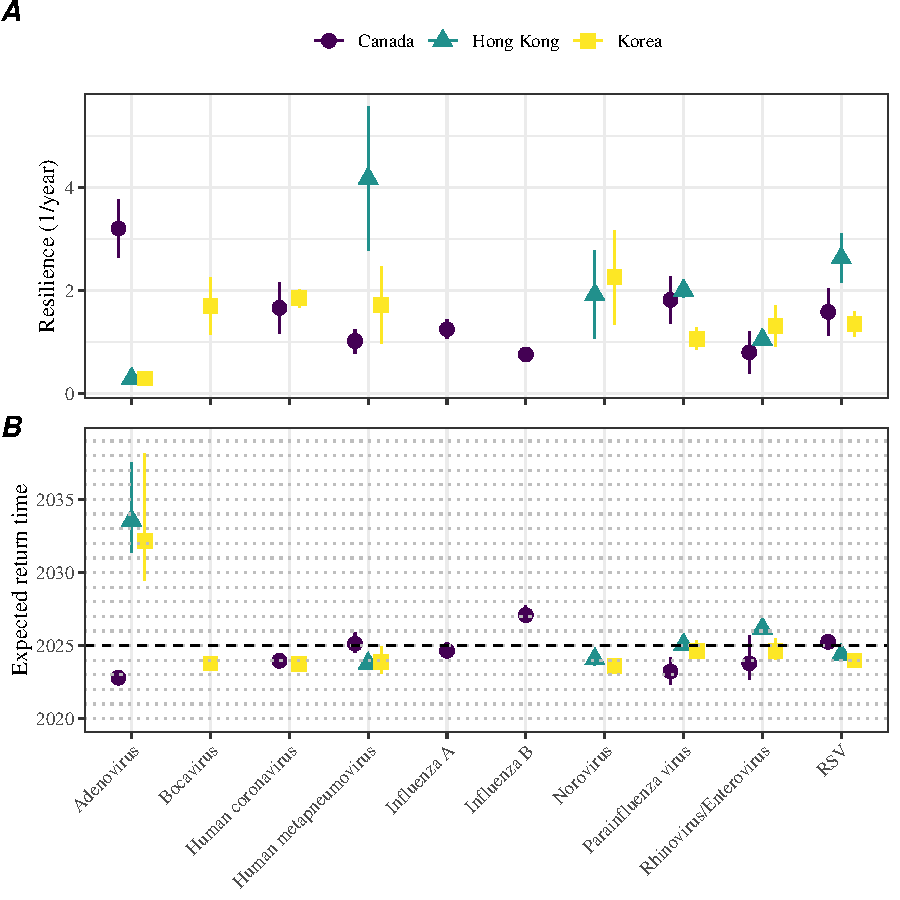
\includegraphics[width=\textwidth]{../figure3/figure3.pdf}
\caption{
\textbf{A schematic diagram explaining the inference of pathogen resilience from synthetic data.}
(A) A realistic example of simulated pandemic perturbations, represented by a relative reduction in transmission.
(B) The impact of the synthetic pandemic perturbation on epidemic dynamics simulated using a SIRS model with demographic stochasticity.
(C) Generating delayed copies of the logged time series allows us to obtain an embedding.
(D) Two dimensional representation of an embedding.
(E) Delayed embedding allows us to calculate the nearest neighbor distance from the empirical attractor, which is determined based on the pre-pandemic time series.
This distance time series can be used to infer pathogen resilience after choosing an appropriate window for linear regression.
}
\end{figure}

Complex changes in the distance from the attractor suggest that estimating pathogen resilience from linear regression will be particularly sensitive to our choice of fitting windows for the regression (Figure 3E).
Therefore, before we tried estimating resilience from real data, we explored an automated window selection criterion for linear regression and test it against randomized, stochastic simulations across a wide range of realistic pandemic perturbation shapes;
in doing so, we also explored optimal choices for embedding dimensions and evaluated our choices for fitting window parameters and embedding dimensions by quantifying correlation coefficients between the estimated resilience and the intrinsic resilience of a seasonally unforced system (Materials and Methods).
Overall, we find large variation in estimation performances with correlation coefficient ranging from 0.21 to 0.61 (Supplementary Figure S7).
In almost all cases, the automated window selection approach outperformed a naive approach that uses the entire time series, starting from the peak distance (Supplementary Figure S7).


% A closer observation of the resulting time series of the distance from the attractor provides three important insights (Figure 3E).
% First, the relaxation of NPIs in realistic settings can cause a false return of the system, as indicated by a rapid decrease in the distance in early 2022 followed by a rapid increase in distance.
% In other words, we need at least several years of data to be able to properly assess the return of system to an attractor.
% Second, complex changes in the distance from the attractor suggests that estimating pathogen resilience from linear regression will likely be sensitive to our choice of fitting windows for the regression.
% Finally, temporal variation in the impact of NPIs on pathogen transmission will affect the intrinsic resilience of the system throughout the NPI period, meaning that the estimated resilience from linear regression will likely reflect some sort of average impact of the NPIs.

Based on the best performing window selection criteria and embedding dimension, we applied this approach to pathogen surveillance data presented in Figure 1 (Materials and Methods).
For each time series, we applied Takens' theorem independently to reconstruct the empirical attractor and obtained the corresponding time series of distances from attractors (Supplementary Figure S8).
Then, we use the automated window selection criterion to fit a linear regression and estimate the empirical resilience for each pathogen in each country (Supplementary Figure S8);
the window selection criterion gave poor regression window for three cases (norovirus in Hong Kong and Korea and Rhinovirus/Enterovirus in the US), leading to unrealistically low resilience estimates, and so we used ad-hoc regression windows instead (Supplementary Figure S9; Materials and Methods).

For all pathogens we consider, resilience estimates fall between $0.4/\mathrm{year}$ and $1.8/\mathrm{year}$ (Figure 4A).
We estimate the mean resilience of common respiratory pathogens to be $0.99/\mathrm{year}$ (95\% CI: $0.80/\mathrm{year}$--$1.18/\mathrm{year}$).
As a reference, this is $\approx 7.5$ times higher than the intrinsic resilience of pre-vaccination measles in England and Wales ($\approx 0.13/\mathrm{year}$).
Finally, resilience estimates for norovirus are comparable to those of common respiratory pathogens: $1.44/\mathrm{year}$ (95\%CI: $1.01/\mathrm{year}$--$1.87/\mathrm{year}$) for Hong Kong and $1.07/\mathrm{year}$ (95\%CI: $0.86/\mathrm{year}$--$1.29/\mathrm{year}$) for Korea.
Based on a simple ANOVA test, we do not find significant differences in resilience estimates across countries ($p=0.25$) or pathogens ($p=0.68$).

\begin{figure}[!th]
\begin{center}
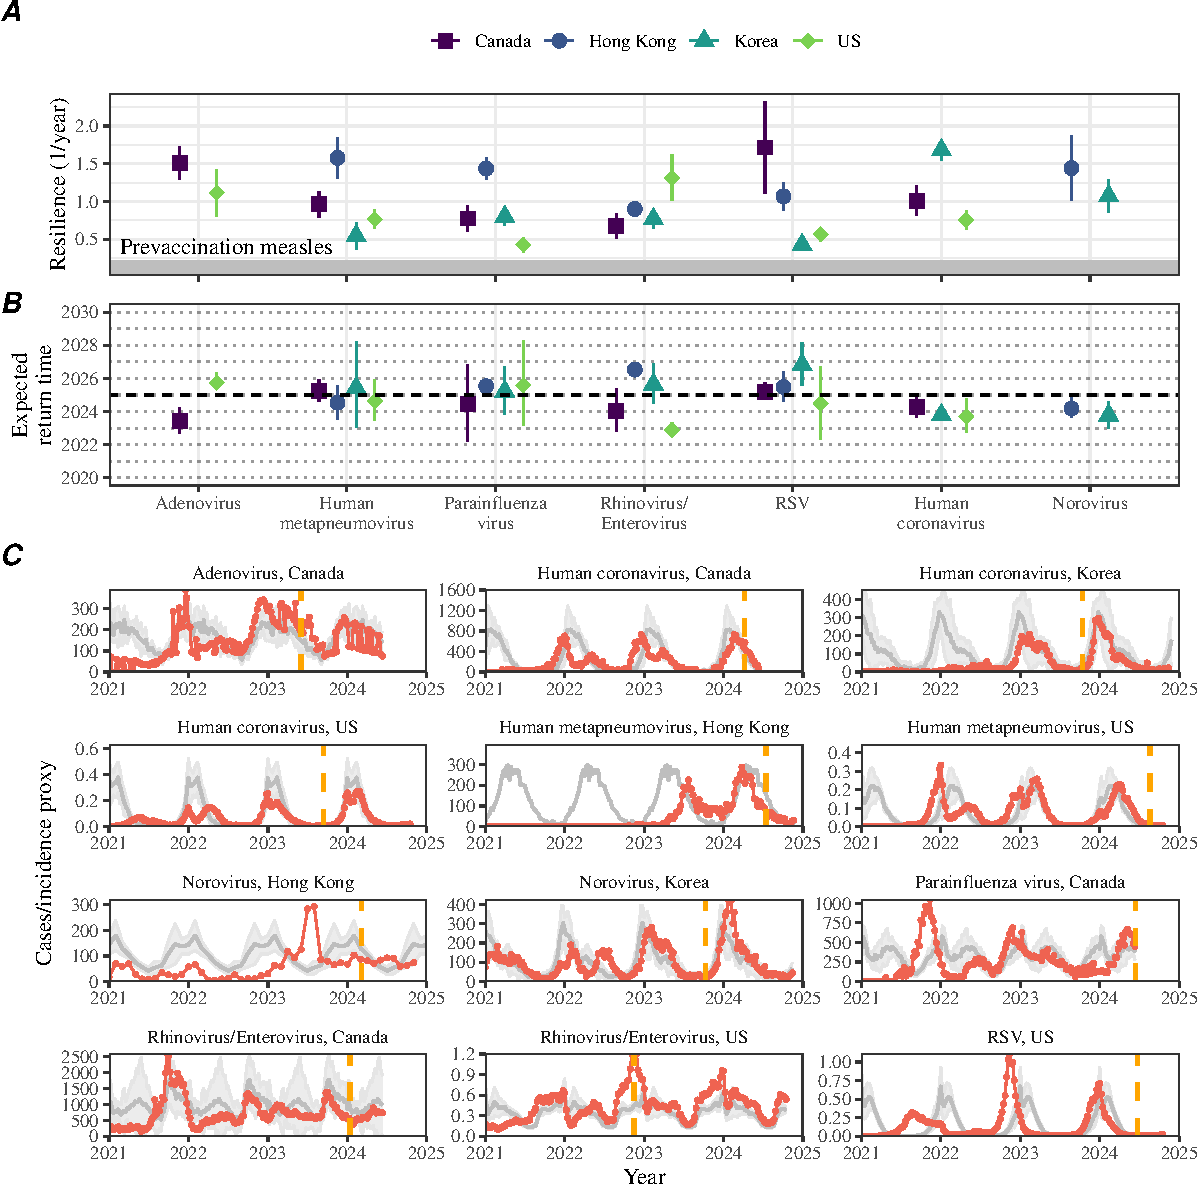
\includegraphics[width=0.8\textwidth]{../figure4/figure4.pdf}
\caption{
\textbf{Summary of resilience estimates and predictions for return time.}
(A) Estimated pathogen resilience.
The gray horizontal line represents the intrinsic resilience of pre-vaccination measles dynamics.
(B) Predicted timing of when each pathogen will return to their pre-pandemic cycles.
The dashed line in panel B indicates the end of 2024 (current observation time).
Error bars represent 95\% confidence intervals.
(C) Observed dynamics for pathogen that are predicted to have returned before the end of 2024.
Red points and lines represent data before 2020.
Gray lines and shaded regions represent the mean seasonal patterns and corresponding 95\% confidence intervals around the mean, previously shown in Figure 1.
Orange vertical lines represent the predicted timing of return.
}
\end{center}
\end{figure}

\swp{You suggested ``I think we probably need to spell out a bit more that long-term changes in the transmission rate (or some other parameter) mean the attractor is permanently different and the distance should remain nonzero'' and I think we've done that enough early on with current revisions so I don't feel like we need to do it again here. Let me know what you think.}
Using resilience estimates, we predicted when each pathogen would hypothetically return to their pre-pandemic dynamics, assuming no long-term change in the attractor.
Specifically, we extend our linear regression fits to distance-from-attractor time series and ask when the predicted regression line will cross a threshold value;
since we relied on nearest neighbor distances, pre-pandemic distances are always greater than zero (Figure 3E), meaning that we can use the mean of pre-pandemic distances as our threshold.

We predict that a return to pre-pandemic cycles would be imminent for most pathogens (Figure 4B).
In particular, we predict that 12 out of 23 pathogens should have already returned before the end of 2024.
For almost all pathogens that are predicted to have returned already, the observed epidemic dynamics show clear convergence towards their pre-pandemic seasonal averages, confirming our predictions (Figure 4C).
However, there are a few exceptions, including norovirus in Hong Kong and Rhinovirus/Enterovirus in the US, where the observed epidemic dynamics in 2024 exhibit clear deviation from their pre-pandemic seasonal averages (Figure 4C).
These observations suggest a possibility that some common respiratory pathogens may have converged to different attractors or are still exhibiting non-equilibrium dynamics.
In contrast, pathogens that are predicted to have not returned yet also show clear differences from their pre-pandemic seasonal averages; as many of these pathogens are predicted to return in 2025--2026, we may be able to test these predictions in near future (Supplementary Figure S10).
Our reconstructions of distance time series and estimates of pathogen resilience and expected return time are generally robust to choices of embedding dimensions (Supplementary Figure S11--12).

\section*{Susceptible host dynamics explain variation in pathogen resilience}

So far, we focused on quantifying pathogen resilience from the observed patterns of pathogen re-emergence following pandemic perturbations.
But what factors determine how resilient a host-pathogen system is?
Here, we use the SIRS model to show that susceptible host dynamics are the key determinants of pathogen resilience.
To do so, we vary the basic reproduction number $\mathcal R_0$, which represents the average number of secondary infections caused by a newly infected individual in a fully susceptible population, and the duration of immunity and compute intrinsic resilience for each parameter.

\begin{figure}[!th]
\begin{center}
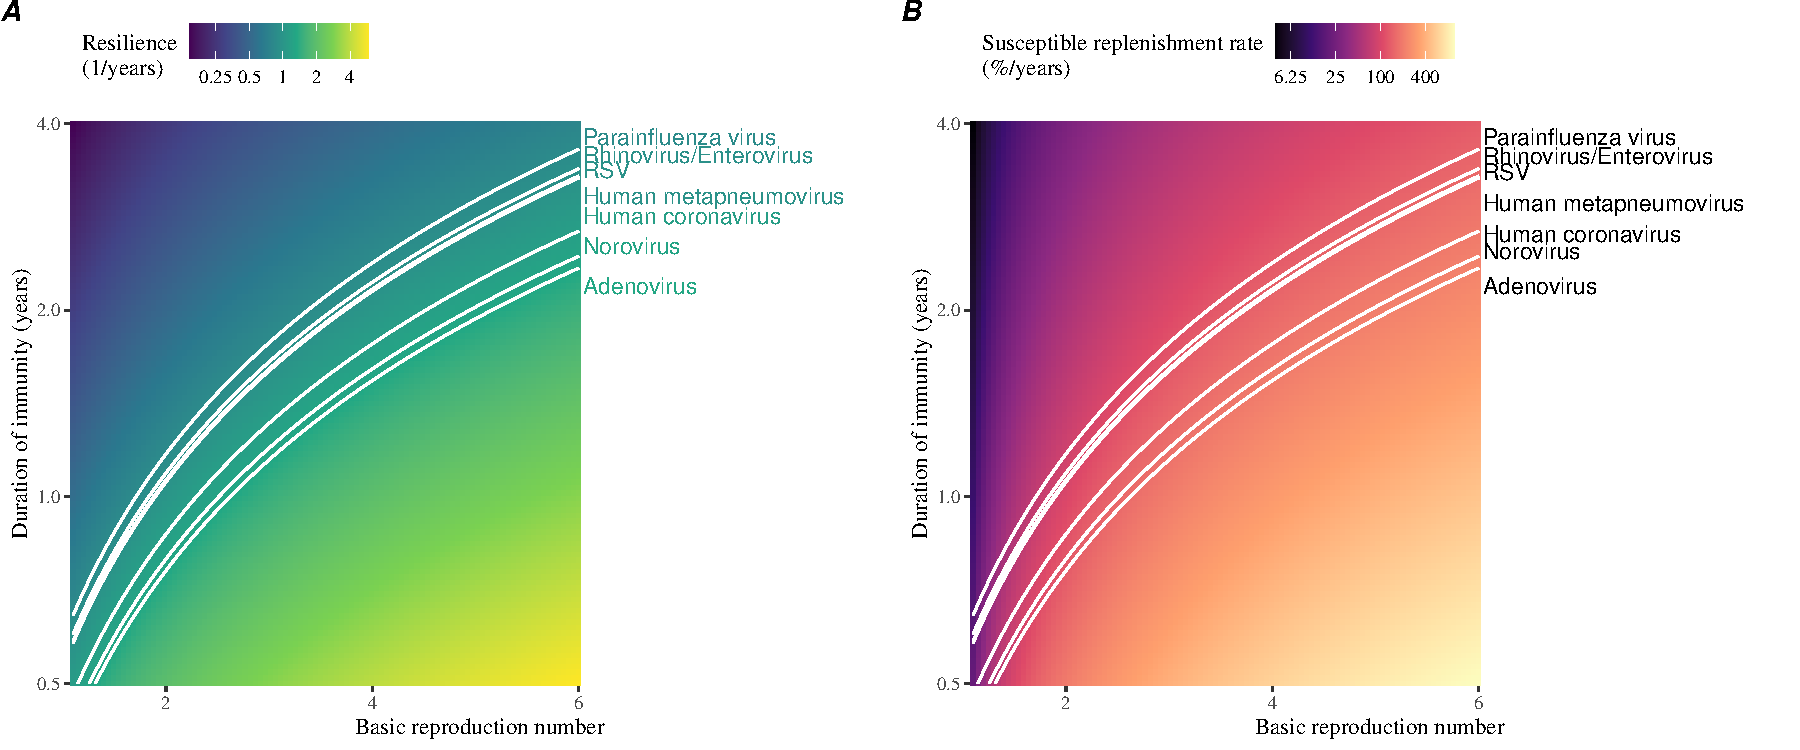
\includegraphics[width=\textwidth]{../figure5/figure5.pdf}
\caption{
\textbf{Linking pathogen resilience to epidemiological parameters and susceptible host dynamics.}
(A) The heat map represents intrinsic resilience as a function of the basic reproduction number $\mathcal R_0$ and the duration of immunity.
(B) The heat map represents per-capita susceptible replenishment rate as a function of the basic reproduction number $\mathcal R_0$ and the duration of immunity.
The standard SIRS model is used to compute intrinsic resilience and per-capita susceptible replenishment rate.
Lines correspond to a set of parameters that are consistent with mean resilience estimates for each pathogen.
Pathogens are ranked based on their mean resilience estimates, averaged across different countries.
}
\end{center}
\end{figure}

We find an increase in $\mathcal R_0$ and a decrease in duration of immunity correspond to an increase in pathogen resilience (Figure 5A).
These variations can be understood in terms of the susceptible host dynamics, where faster per-capita susceptible replenishment rate causes the system to be more resilient (Figure 5B).
This rate can be expressed as a ratio between absolute rate at which new susceptibles enter the population and the equilibrium number of susceptible individuals in the population, $\bar{S}$.
Therefore, both higher $\mathcal R_0$ and shorter duration of immunity can drive faster per-capita susceptible replenishment rate (Figure 5B), especially because higher $\mathcal R_0$ leads to lower $\bar{S}$.

We can also rank different pathogens based on the average values of empirical resilience computed previously, which allows us to determine a set of parameters that are consistent with the estimated resilience (Figure 5A).
Across all pathogens we consider, except for bocavirus and norovirus, we estimate that the average duration of immunity is likely to be short ($<4$ years) across a plausible range of $\mathcal R_0$ ($<6$).
These rankings further allow us to map each pathogen onto a set of SIRS parameters that are consistent with its empirical resilience (Figure 5A) and obtain a plausible range of susceptible replenishment rates for each pathogen (Figure 5B).
However, we note that there is no one-to-one correspondence between susceptible replenishment rates and pathogen resilience, leading to a wide uncertainty in the estimates for susceptible replenishment rates (Figure 5B).

\section*{Pathogen resilience determines sensitivity to stochastic perturbations}

Beyond the pandemic perturbations, we expect host-pathogen systems to experience continued perturbations of varying degrees from changes in epidemiological conditions, such as human behavior, climate, and viral evolution.
These perturbations can also arise from demographic stochasticity, which is inherent to any ecological systems.
Here, we use a seasonally unforced SIRS model with birth/death to explore how resilience of a host-pathogen system determines the sensitivity to perturbations caused by demographic stochasticity (Materials and Methods).

\begin{figure}[!th]
\begin{center}
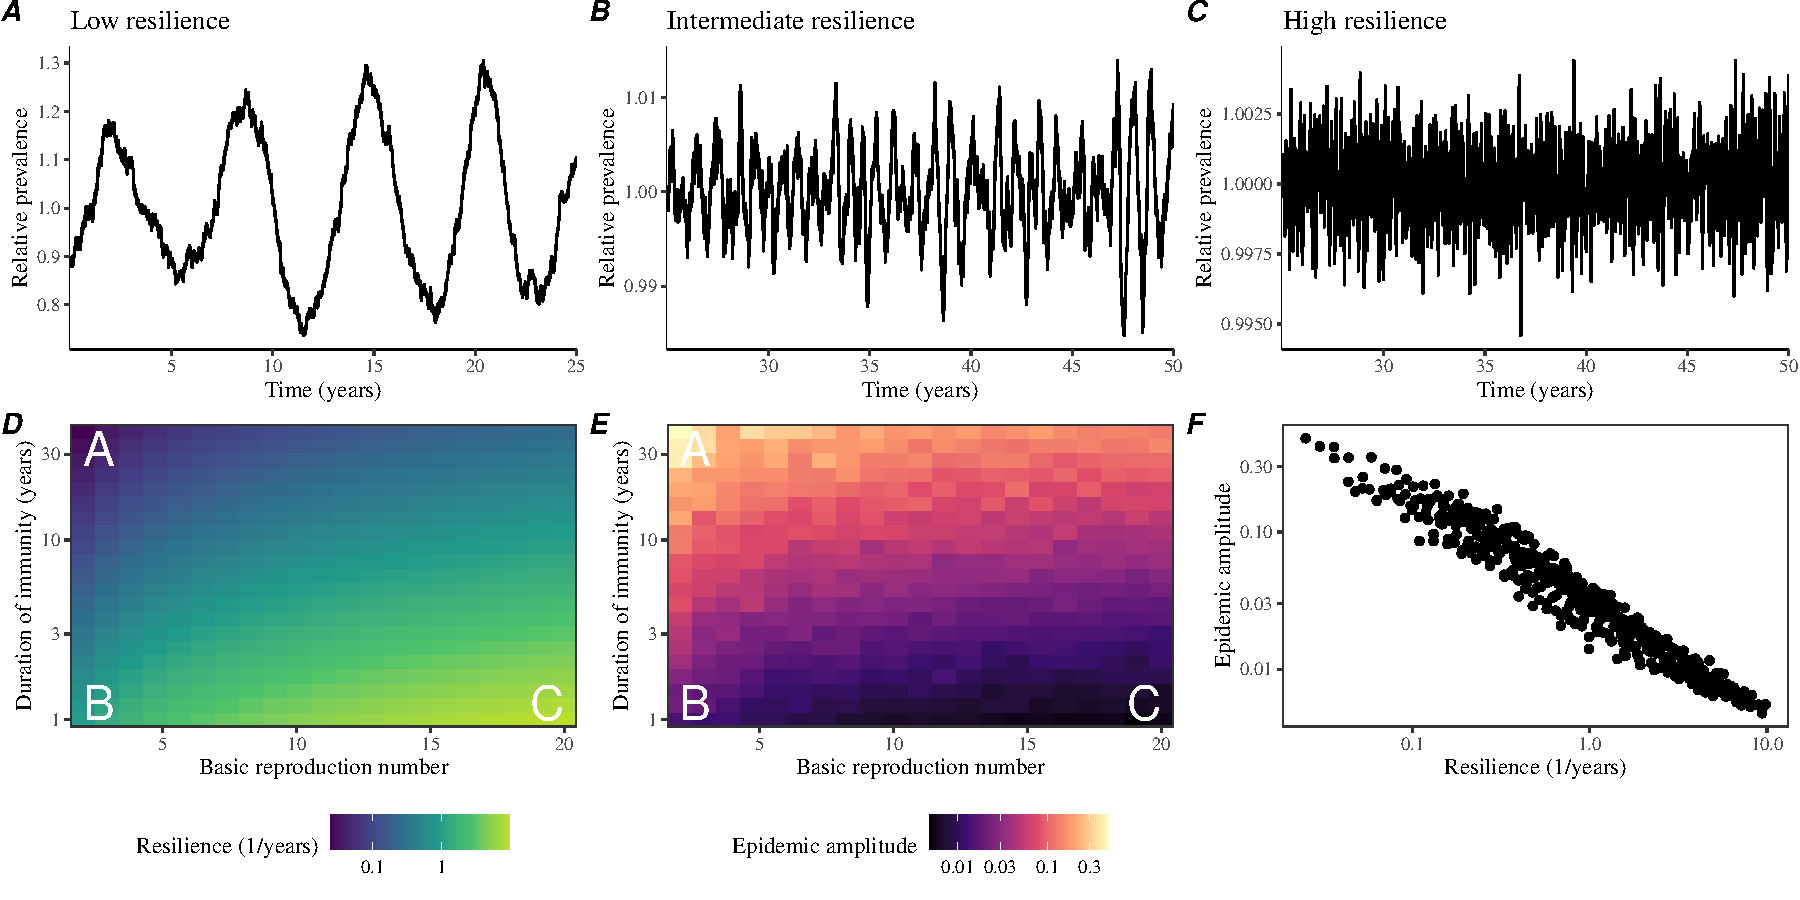
\includegraphics[width=\textwidth]{../figure6/figure_persistence_noise.pdf}
\caption{
\textbf{Linking resilience of a host-pathogen system to its sensitivity to stochastic perturbations.}
(A--C) Epidemic trajectories of a stochastic SIRS model across three different resilience values: low, intermediate, and high.
The relative prevalence was calculated by dividing infection prevalence by its mean value.
(D) The heat map represents the intrinsic resilience of a system as a function of the basic reproduction number $\mathcal R_0$ and the duration of immunity.
(E) The heat map represents the epidemic amplitude as a function of the basic reproduction number $\mathcal R_0$ and the duration of immunity.
The epidemic amplitude corresponds to $(\max I - \min I)/(2 \bar{I})$, where $\bar{I}$ represents the mean prevalence.
(F) The relationship between pathogen resilience and epidemic amplitude.
}
\end{center}
\end{figure}

We find that resilience of a host-pathogen system determines  the amount of deviation from the deterministic trajectory caused by demographic stochasticity, with less resilient systems experiencing larger deviations (Figure 6).
Notably, less resilience systems also exhibit slower epidemic cycles; the periodicity of this epidemic cycle matches those predicted by the intrinsic periodicity of the system (Supplementary Figure S13).
These conclusions are robust for the seasonally forced SIRS model (Supplementary Figure S14),

\section*{Discussion}

The pandemic interventions have caused major disruptions to circulation patterns of both respiratory and non-respiratory pathogens, adding challenges to predicting their future dynamics \citep{baker2020impact,gomez2021uncertain,koltai2022determinants,park2024predicting}.
However, these perturbations offer large-scale natural experiments for understanding how different pathogens respond to perturbations.
In this study, we showed that pathogen re-emergence patterns following pandemic perturbations can be characterized through the lens of ecological resilience.
We showed that variation in pathogen resilience can be explained by the differences in susceptible host dynamics, where faster replenishment of the susceptible pool corresponds to a more resilient host-pathogen system.
Finally, we showed that pathogen resilience also determines the sensitivity to stochastic perturbations.

We analyzed case time series of common respiratory infections and norovirus infections from Canada, Hong Kong, Korea, and the US to estimate their resilience.
Overall, we estimated the resilience of these pathogens to range from $0.4/\mathrm{year}$ to $1.8/\mathrm{year}$, which is 3--14 times more resilient than prevaccination measles.
These resilience estimates indicate that common respiratory pathogens and norovirus likely exhibit faster susceptible replenishment and are therefore more persistent, indicating potential challenges in controlling these pathogens.

Based on our resilience estimates, we made phenomenological predictions about when each pathogen will return to their endemic cycles.
For the most part, we accurately predicted which pathogens should have already returned before the end of 2024.
However, there were few exceptions (i.e., norovirus in Hong Kong and rhinovirus/enterovirus in the US), suggesting a possibility that these may have converged to different endemic cycles compared to their pre-pandemic epidemic patterns.
These changes may reflect changes in surveillance or actual shift in the dynamics, caused by permanent changes in behavior or population-level immunity.
While it may seem unlikely that permanent changes in behavior would only affect a few pathogens and not others, we cannot rule out this possibility given heterogeneity in the age of infection across different respiratory pathogens \citep{radin2014epidemiology,lv2024epidemiological}.
Differences in the mode of transmission between respiratory vs gastrointestinal pathogens may also contribute to the differences in responses to pandemic perturbations.
However, it is unclear why norovirus dynamics in Korea seemed to have returned, whereas those in Hong Kong have not.

For almost half of the pathogens we considered, we predicted that their return to original epidemic patterns is imminent.
We will need a few more years of data to test whether these pathogens will eventually return to their original dynamics or eventually converge to a different attractor.
Overall, these observations echo earlier studies that highlighted the long-lasting impact of pandemic perturbations \citep{baker2022long,caini2024probable,chen2024covid,park2024predicting}. 

We showed that susceptible host dynamics shape pathogen resilience, where faster replenishment of the susceptible population causes the pathogen to be more resilient.
For simplicity, we focus on waning immunity and birth as the main drivers of the susceptible host dynamics but other mechanisms can also contribute to the replenishment of the susceptible population.
In particular, pathogen evolution, especially the emergence of antigenically novel strains, can cause effective waning of immunity in the population;
therefore, we hypothesize that faster rates of antigenic evolution can also cause a pathogen to be more resilient.
Future studies should explore the relationship between the rate of evolution and resilience for antigenically evolving pathogens.

Quantifying pathogen resilience also offers novel approaches to validating population-level epidemiological models.
So far, most of model validation in infectious disease ecology is based on the ability of a model to reproduce the observed epidemic dynamics and to predict future dynamics \citep{grenfell2002dynamics,bhattacharyya2015cross,pitzer2015environmental,dean2018human,pons2018serotype}.
However, many models can perform similarly under these criteria.
For example, two major RSV models have been proposed to explain biennial epidemic patterns: (1) a stage- and age-structured model that allows disease severity to vary with number of past infections and age of infection \citep{pitzer2015environmental} and (2) a pathogen-interaction model that accounts for cross immunity between RSV and human metapnuemovirus \citep{bhattacharyya2015cross}.
Since both models can accurately reproduce the observed epidemic patterns, standard criteria for model validation do not allow us to distinguish between these two models from population-level data alone.
Instead, it would be possible to measure the empirical resilience of each model by simulating various perturbations and compare them to estimates of empirical resilience from data, using pandemic NPIs as an opportunity.
% Future studies should further investigate using pathogen resilience for validating epidemic models.

There are several limitations to our work.
First, we did not extensively explore other approaches to reconstructing the attractor.
Recent studies showed that more sophisticated approaches, such as using non-uniform embedding, can provide more robust reconstruction for noisy data \citep{tan2023selecting}.
In the context of causal inference, choices about embedding can have major impact on the resulting inference \citep{cobey2016limits}.
Our resilience estimates are likely overly confident given a lack of uncertainties in attractor reconstruction as well as the simplicity of our statistical framework.
Nonetheless, as illustrated in our sensitivity analyses, inferences about pathogen resilience in our SIRS model appear to be robust to decisions about embedding lags and dimensions---this is because tracking the rate at which the system approaches the attractor is likely a much simpler problem than making inferences about causal directionality.
Short pre-pandemic time series also limit our ability to accurately reconstruct the attractor and contribute to the crudeness of our resilience estimates;
although this is less likely a problem for respiratory pathogens that are strongly annual, our attractor reconstruction may be inaccurate for those exhibiting multi-annual cycles, such as adenovirus in Hong Kong and Korea.
Despite these limitations, our qualitative prediction that common respiratory pathogens are more resilient than prevaccination measles is also likely to be robust, given how rapid many respiratory pathogens returned to their original cycles following pandemic NPIs.
% Despite these limitations, our study illustrates the utility of quantifying pathogen resilience for understanding how different pathogens respond to perturbations.

Predicting the impact of anthropogenic changes on infectious disease dynamics is a fundamental aim of infectious disease research in a rapidly changing world.
Our study illustrates that quantifying pathogen resilience can help us understand how infectious disease pathogens respond to major perturbations caused by NPIs.
More broadly, a detailed understanding of the determinants of pathogen resilience may offer unique insights into pathogen persistence and controllability.

\section*{Materials and Methods}

\subsection*{Data}

We gathered time series on respiratory infections from Canada, Hong Kong, Korea, and United States (US).
As a reference, we also included time series data on norovirus infections for available countries.
In contrast to respiratory pathogens, we expect gastrointestinal viruses, such as norovirus, to be differently affected by pandemic perturbations.

Weekly time series of respiratory infection cases in Canada comes from a publicly available website by the Respiratory Virus Detection Surveillance System, which collect data from select laboratories across Canada \citep{phac}.
Weekly time series of respiratory infection cases in Hong Kong comes from a publicly available website by the  Centre for Health Protection, Department of Health \citep{hkdata}.
Weekly time series of acute respiratory infection cases in Korea comes from a publicly available website by the Korea Disease Control and Prevention Agency \citep{kordata}.
Finally, weekly time series of respiratory infection cases in the US were obtained from the National Respiratory and Enteric Virus Surveillance System.

\subsection*{Data processing}

For all time series, we rounded every year to 52 weeks by taking the average number of cases and tests between the 52nd and 53rd week.
We also rescale all time series to account for changes in testing patterns, which are then used for the actual analysis.

Canada: To account for an increase in testing from 2013 to 2024, we calculate a 2 year moving average for the number of tests for each pathogen, which we use as a proxy for testing effort.
Then, we divide the smoothed testing patterns by the smoothed value at the final week such that the testing effort has a maximum of 1.
We then divide weekly cases by the testing effort to obtain a scaled case time series.
A similar approach was used earlier for the analysis of RSV time series in the US \citep{pitzer2015environmental}.

Hong Kong: We also apply the same scaling procedure to the time series as we did for Canada.
For Hong Kong, we only adjust for testing efforts up to the end of 2019 because there was a major reduction in testing for common respiratory pathogens since 2020.

Korea: While we do not have information on testing, the reported number of respiratory infections consistently increased from 2013 to the end of 2019, which we interpreted as changes in testing patterns.
Since we do not have testing numbers, we used the weekly sum of all acute respiratory viral infection cases as a proxy for testing, which were further smoothed with moving averaged and scaled to have a maximum of 1.
For Korea, we also only adjust for testing efforts up to the end of 2019.

US: In the US, there has been a large increase in testing against some respiratory pathogens, especially RSV, which could not be corrected for through simple scaling.
Instead, we derive an incidence proxy by multiplying the test positivity with influenza-like illness positivity, which is taken from \url{https://gis.cdc.gov/grasp/fluview/fluportaldashboard.html}.
This method of estimating an incidence proxy has been recently applied in the analysis of seasonal coronaviruses \citep{kissler2020projecting} and \textit{Mycoplasma pneumoniae} infections \citep{park2024predicting}.
Detailed assumptions and justifications are provided in \citep{goldstein2011predicting}.

\subsection*{Estimating pathogen resilience}

In order to measure pathogen resilience from surveillance data, we first reconstruct the empirical pre-pandemic attractor of the system using Takens' embedding theorem \citep{takens2006detecting}.
Specifically, for a given pathogen, we take the pre-pandemic (before 2020) case time series $C(t)$ and reconstruct the attractor using delayed embedding with a uniform delay of $\tau$ and dimension $M$:
\begin{equation}
X_{\tau,m}(t) = \langle\log(C(t)+1), \log(C(t-\tau)+1), \dots, \log(C(t-(M-1)\tau)+1)\rangle.
\end{equation}
Here, the delay $\tau$ is determined by calculating the autocorrelation of the logged pre-pandemic time series and asking when the autocorrelation crosses 0 for the first time \citep{tan2023selecting};
a typical delay for for an annual outbreak is around 13 weeks.

Then, for a given delay $\tau$, we determine the embedding dimension $M$ using the false nearest neighbors approach \citep{kennel1992determining,tan2023selecting}.
To do so, we start with an embedding dimension $e$ and construct a set of points $A_{\tau,e}= \{X_{\tau,e}(t) | t < 2020\}$.
Then, for each point $X_{\tau,e}(t)$, we determine the nearest neighbor from the set $A_{\tau,e}$, which we denote $X_{\tau,e}(\tsub{t}{nn})$ for $t \neq \tsub{t}{nn}$.
Then, if the distance between these two points on $e+1$ dimension, $D_{\tau,e+1}(t) = ||X_{\tau,e+1}(\tsub{t}{nn})-X_{\tau,e+1}(t)||_2$, is larger than their distance on $e$ dimension, $D_{\tau,e}(t) = ||X_{\tau,e}(\tsub{t}{nn})-X_{\tau,e}(t)||_2$, these two points are deemed to be false nearest neighbors;
specifically, we use a threshold $R$ for the ratio between two distances $D_{\tau,e+1}(t)/D_{\tau,e}(t)$ to determine false nearest neighbors.
In the main text, we determine the embedding dimension based on the first dimension without any false nearest neighbors for $R=10$.
In Supplementary Materials, we impose $R=5$ to select for higher dimensions.
Once we determine the embedding lag $\tau$ and dimension $M$, we apply the embedding to the entire time series and calculate the nearest neighbor distance against the attractor $A_{\tau,M}$ to obtain a time series of distance from the attractor $D_{\tau,M}(t)$.

From a time series of distances from the attractor, we estimate pathogen resilience by fitting a linear regression to an appropriate window.
To automatically select the fitting window, we begin by smoothing the distance time series using locally estimated scatterplot smoothing (LOESS) to obtain $\hat{D}_{\tau,M}(t)$, where the smoothing is performed on a log scale and exponentiated afterwards.
Then, we determine threshold values ($\tsub{T}{start}$ and $\tsub{T}{end}$) for the smoothed distances and choose the fitting window based on when $\hat{D}_{\tau,M}(t)$ crosses these threshold values for the first time.
These thresholds are determined by first calculating maximum distance,
\begin{equation}
\max \hat{D} = \max \hat{D}_{\tau,M}(t),
\end{equation}
and mean pre-pandemic distance,
\begin{equation}
\tsub{\hat{D}}{mean} = \frac{1}{N_{t<2020}} \sum_{t < 2020} \hat{D}_{\tau,M}(t),
\end{equation}
as a reference, and then dividing their ratios into 10 equal bins:
\begin{align}
\tsub{T}{start} &= \tsub{\hat{D}}{mean} \times \left(\frac{\max \hat{D}}{\tsub{\hat{D}}{mean}} \right)^{9/10}\\
\tsub{T}{end} &= \tsub{\hat{D}}{mean} \times \left(\frac{\max \hat{D}}{\tsub{\hat{D}}{mean}} \right)^{1/10}
\end{align}
This allows us to discard the initial period during which the distance increases (from the introduction of intervention measures) and the final period during which the distance plateaus (as the system reaches an attractor).
The fitting window is determined based on when the smoothed distance $\hat{D}_{\tau,M}(t)$ crosses these threshold values for the first time; then, we fit a linear regression to logged (unsmoothed) distances $\log D_{\tau,M}(t)$ using that window.

\subsection*{Mathematical modeling}

Throughout the paper, we use a series of mathematical models to illustrate the concept of pathogen resilience and to understand the determinants of pathogen resilience.
In general, the intrinsic resilience for a given system is given by the largest real part of the eigenvalues of the linearized system at endemic equilibrium.
Here, we focus on the SIRS model with demography and present the details of other models in Supplementary Materials.
The SIRS (Susceptible-Infected-Recovered-Susceptible) model is the simplest model that allows for waning of immunity, where recovered (immune) individuals are assumed to become fully susceptible after an average of $1/\delta$ time period.
The dynamics of the SIRS model is described by the following set of differential equations:
\begin{align}
\frac{\dd S}{\dd t} &= \mu - \beta(t) SI - \mu S + \delta R \\
\frac{\dd I}{\dd t} &= \beta(t) SI - (\gamma + \mu) I \\
\frac{\dd R}{\dd t} &= \gamma I - (\delta + \mu) R \\
\end{align}
where $\mu$ represents the birth/death rate, $\beta(t)$ represents the time-varying transmission rate, and $\gamma$ represents the recovery rate.
The basic reproduction number $\mathcal R_0(t) = \beta(t)/(\gamma + \mu)$ is defined as the average number of secondary infections that a single infected individual would cause in a fully susceptible population at time $t$ and measures the intrinsic transmissibility of a pathogen.

When we first introduce the idea of pathogen resilience (Figure 2), we impose sinusoidal changes to the transmission rate to account for seasonal transmission:
\begin{equation}
\beta(t) = b_1 (1 + \theta \cos(2 \pi (t-\phi))) \alpha(t),
\end{equation}
where $b_1$ represents the baseline transmission rate, $\theta$ represents the seasonal amplitude, and $\phi$ represents the seasonal offset term.
Here, we also introduce an extra multiplicative term $\alpha(t)$ to account for the impact of pandemic NPIs, where $\alpha(t) < 1$ indicates transmission reduction.
Figure 2A and 2B are generated assuming $b_1 = 3 \times (365/7+1/50)/\mathrm{years}$, $\theta=0.2$, $\phi=0$, $\mu=1/50/\mathrm{years}$, $\gamma=365/7/\mathrm{years}$, and $\delta=1/2/\mathrm{years}$,
In Figure 2A, we impose a 50\% transmission reduction for 6 months from 2020:
\begin{equation}
\alpha(t) = \begin{cases}
0.5 & 2020 \leq t< 2020.5\\
1 & \textrm{otherwise}
\end{cases}
\end{equation}
In Figure 2B, we impose a 50\% transmission reduction for 6 months from 2020 and a permanent 10\% reduction onward:
\begin{equation}
\alpha(t) = \begin{cases}
1 & t < 2020\\
0.5 & 2020 \leq t < 2020.5\\
0.9 & 2020.5 \leq t
\end{cases}
\end{equation}
In both scenarios, we simulate the SIRS model from the following initial conditions ($S(0) = 1/\mathcal R_0$, $I(0) = 1\times 10^{-6}$, and $R(0) = 1 - S(0) - I(0)$) from 1900 until 2030.

To measure the empirical resilience of the SIR model (Figure 2C and 2F), we compute the normalized distance between post-intervention susceptible and logged infected proportions and their corresponding pre-intervention values at the same time of year:
\begin{equation}
\sqrt{\left(\frac{S(t) - \tsub{S}{pre}(t)}{\sigma_S}\right)^2 + \left(\frac{\log I(t) - \log \tsub{I}{pre}(t)}{\sigma_{\log I}}\right)^2},
\end{equation}
where $\sigma_S$ and $\sigma_{\log I}$ represent the standard deviation in the pre-intervention susceptible and logged infected proportions.
We normalize the differences in susceptible and logged infected proportions to allow both quantities to equally contribute to the changes in distance from the attractor.
We used logged prevalence, instead of absolute prevalence, in order to capture epidemic dynamics in deep troughs during the intervention period.
In Supplementary Materials, we also compare how the degree of seasonal transmission affects empirical resilience by varying $\theta$ from 0 to 0.4; when we assume no seasonality ($\theta = 0$), we do not normalize the distance because the standard deviation of pre-intervention dynamics are zero. 

Finally, we use the SIRS model to understand how underlying epidemiological parameters affect pathogen resilience and link this relationship to underlying susceptible host dynamics.
For the simple SIRS model without seasonal transmission ($\theta = 0$), the intrinsic resilience corresponds to
\begin{equation}
-\frac{\mathrm{Re}(\lambda)}{2} = \frac{\delta + \beta I^{\ast} + \mu}{2}.
\end{equation}
Here, $I^{\ast}$ represents the prevalence at endemic equilibrium:
\begin{equation}
I^{\ast} = \frac{(\delta + \mu)(\beta - (\gamma + \mu))}{\beta(\delta + \gamma + \mu)}.
\end{equation}
The susceptible replenishment rate is given by
\begin{equation}
\tsub{S}{replenish} = \frac{\mu + \delta R}{S^\ast},
\end{equation}
where $S^\ast = 1/\mathcal R_0$ represents the equilibrium proportion of susceptible individuals.
We vary the basic reproduction number $\mathcal R_0$ between 1.1 to 6 and the average duration of immunity $1/\delta$ between 2 to 80 years, and compute these two quantities.
In doing so, we fix all other parameters: $\mu=1/80/\mathrm{years}$ and $\gamma=365/7/\mathrm{years}$.

\section*{Data availability}

\section*{Funding}

\pagebreak

\setcounter{figure}{0}
\setcounter{equation}{0}
\renewcommand{\thefigure}{S\arabic{figure}}
\renewcommand{\theequation}{S\arabic{equation}}

\section*{Supplementary Text}

\subsection*{Resilience of a stage-structured system.}

In Figure 2G--I, we use a more realistic, stage-structured model to illustrate how transient phenomena can cause the system to slow down.
Specifically, we use the stage-structured RSV model proposed by \citep{pitzer2015environmental}, which assumes that subsequent reinfections cause an individual to become less susceptible and transmissible than previous infections.
The model dynamics can be described as follows:
\begin{align}
\frac{\dd M}{\dd t} &= \mu - (\omega + \mu) M\\
\frac{\dd S_0}{\dd t} &= \omega M - (\lambda(t) + \mu) S_0\\
\frac{\dd I_1}{\dd t} &= \lambda(t) S_0 - (\gamma_1 + \mu) I_1\\
\frac{\dd S_1}{\dd t} &= \gamma_1 I_1 - (\sigma_1 \lambda(t) + \mu) S_1\\
\frac{\dd I_2}{\dd t} &= \sigma_1 \lambda(t) S_1 - (\gamma_2 + \mu) I_2\\
\frac{\dd S_2}{\dd t} &= \gamma_2 I_2 - (\sigma_2 \lambda(t) + \mu) S_2\\
\frac{\dd I_3}{\dd t} &= \sigma_2 \lambda(t) S_2 - (\gamma_3 + \mu) I_3\\
\frac{\dd S_3}{\dd t} &= \gamma_3 I_3 - (\sigma_3 \lambda(t) + \mu) S_3 + \gamma_4 I_4\\
\frac{\dd I_4}{\dd t} &= \sigma_3 \lambda(t) S_3 - (\gamma_4 + \mu) I_4\\
\end{align}
where $M$ represents the proportion of individuals who are maternally immune;
$S_i$ represents the proportion of individuals who are susceptible after $i$ prior infections;
$I_i$ represents the proportion of individuals who are currently (re)-infected with their $i$-th infection;
$\mu$ represents the birth and death rates;
$1/\omega$ represents the mean duration of maternal immunity;
$1/\gamma_i$ represents the mean duration of infection;
$\lambda(t)$ represents the force of infection;
and $\sigma_i$ represents the reduction in susceptibility for the $i$-th reinfection.
The force of infection is modeled using a sinusoidal function:
\begin{align}
\beta(t) &= b_1 (1 + \theta \cos(2 \pi (t-\phi))) \alpha(t)\\
\lambda(t) &= \beta (I_1 + \rho_1 I_2 + \rho_2 (I_3 + I_4)), 
\end{align}
where $b_1$ represents the baseline transmission rate; $\theta$ represents the seasonal amplitude; $\phi$ represents the seasonal offset term; $\alpha(t)$ represents the intervention effect; and $\rho_i$ represents the impact of immunity on transmission reduction.
We use the following parameters to simulate the impact of interventions on epidemic dynamics \citep{pitzer2015environmental}: $b_1 = 9 \times (365/10+1/80)/\mathrm{years}$, $\theta = 0.2$, $\phi = -0.1$, $\omega=365/112/\mathrm{years}$, $\gamma_1=365/10/\mathrm{years}$, $\gamma_2=365/7/\mathrm{years}$, $\gamma_3=365/5/\mathrm{years}$, $\sigma_1 = 0.76$, $\sigma_2 = 0.6$, $\sigma_3 = 0.4$, $\rho_1 = 0.75$, $\rho_2 = 0.51$, and $\mu = 1/80/\mathrm{years}$.
We assume a 50\% transmission reduction for 6 months from 2020:
\begin{equation}
\alpha(t) = \begin{cases}
0.5 & 2020 \leq t< 2020.5\\
1 & \textrm{otherwise}
\end{cases}
\end{equation}
The model is simulated from 1900 to 2030 using the following initial conditions: $M=0$, $S_0=1/\mathcal R_0-I_1$, $I_1=1\times 10^{-6}$, $S_1=1-1/\mathcal R_0$, $I_2=0$, $S_2=0$, $I_3=0$, $S_3=0$, and $I_4=0$.
For the phase plane analysis (Figure 2H) and distance analysis (Figure 2I), we rely on the average susceptibility,
\begin{equation}
\bar{S} = S_0 + \sigma_1 S_1 + \sigma_2 S_2 + \sigma_3 S_3,
\end{equation}
and total prevalence,
\begin{equation}
\tsub{I}{total} = I_1 + I_2 + I_3 + I_4.
\end{equation}
These quantities are used to compute the normalized distance from the attractor, as described in the main text.

\subsection*{Resilience of a multistrain system.}

We use a simple two-strain model to show that a multistrain host-pathogen system that is coupled through cross immunity can be described by a single resilience value.
The model dynamics can be described as follows \citep{bhattacharyya2015cross}: 
\begin{align}
\frac{\dd S}{\dd t} &= \mu - \mu S - (\lambda_1 + \lambda_2) S + \rho_1 R_1 + \rho_2 R_2 \\
\frac{\dd I_1}{\dd t} &= \lambda_1 S - (\gamma_1 + \mu) I_1 \\
\frac{\dd I_2}{\dd t} &= \lambda_2 S - (\gamma_2 + \mu) I_2 \\
\frac{\dd R_1}{\dd t} &= \gamma_1 I_1 - \lambda_2 \epsilon_{21} R_1 - \rho_1 R_1 + \rho_2 R - \mu R_1\\
\frac{\dd R_2}{\dd t} &= \gamma_2 I_2 - \lambda_1 \epsilon_{12} R_2 - \rho_2 R_2 + \rho_1 R - \mu R_2\\
\frac{\dd J_1}{\dd t} &= \lambda_1 \epsilon_{12} R_2 - (\gamma_1 + \mu) J_1\\
\frac{\dd J_2}{\dd t} &= \lambda_2 \epsilon_{21} R_1 - (\gamma_2 + \mu) J_2\\
\frac{\dd R}{\dd t} &= \gamma_1 J_1 + \gamma_2 J_2 - \rho_1 R - \rho_2 R - \mu R
\end{align}
where $S$ represents the proportion of individuals who are fully susceptible to infections by both strains;
$I_1$ represents the proportion of individuals who are infected with strain 1 without prior immunity;
$I_2$ represents the proportion of individuals who are infected with strain 2 without prior immunity;
$R_1$ represents the proportion of individuals who are fully immune against strain 1 and partially susceptible to reinfection by strain 2;
$R_2$ represents the proportion of individuals who are fully immune against strain 2 and partially susceptible to reinfection by strain 1;
$J_1$ represents the proportion of individuals who are infected with strain 1 with prior immunity against strain 2;
$J_2$ represents the proportion of individuals who are infected with strain 2 with prior immunity against strain 1;
$R$ represents the proportion of individuals who are immune to infections from both strains;
$\mu$ represents the birth/death rate;
$\lambda_1$ and $\lambda_2$ represent the force of infection from strains 1 and 2, respectively;
$\rho_1$ and $\rho_2$ represent the waning immunity rate;
$\gamma_1$ and $\gamma_2$ represent the recovery rate;
$\epsilon_{21}$ and $\epsilon_{12}$ represent the susceptibility to reinfection with strains 2 and 1, respectively, given prior immunity from infection with strains 1 and 2, respectively. 
The force of infection is modeled as follows:
\begin{align}
\beta_1 &= b_1 (1 + \theta_1 \sin(2 \pi (t-\phi_1))) \alpha(t)\\
\beta_2 &= b_2 (1 + \theta_2 \sin(2 \pi (t-\phi_2))) \alpha(t)\\
\lambda_1 &= \beta_1 (I_1 + J_1)\\
\lambda_2 &= \beta_2 (I_2 + J_2)
\end{align}
In Supplementary Figures S2--S4, we assume the following parameters:
$b_1 = 2 \times 52/\mathrm{years}$, $b_2 = 4 \times 52/\mathrm{years}$, $\phi_1 = \phi_2 = 0$, $\epsilon_{12} = 0.9$, $\epsilon_{21} = 0.5$,
$\gamma_1 = \gamma_2 = 52/\mathrm{years}$, $\rho_1 = \rho_2 = 1/\mathrm{years}$, and $\mu=1/70/\mathrm{years}$.
For all simulations, we assume a 50\% transmission reduction for 6 months from 2020:
\begin{equation}
\alpha(t) = \begin{cases}
0.5 & 2020 \leq t< 2020.5\\
1 & \textrm{otherwise}
\end{cases}
\end{equation}
The seasonal amplitude $\theta$ is varied from 0 to 0.4.
All simulations were ran from 1900 to 2030 with following initial conditions: 
$S(0) = 1 - 2\times 10^{-6}$, $I_1(0) = 1 \times 10^{-6}$, $I_2(0) = 1 \times 10^{-6}$, $R_1(0) = 0$, $R_2(0) = 0$, $J_1(0) = 0$, $J_2(0) = 0$, and $R(0) = 0$.

We consider three scenarios for measuring pathogen resilience: (1) we only have information about strain 1, (2) we only have information about strain 2, and (3) we are unable to distinguish between strains.
In the first two scenarios (see panels A--C for strain 1 and panels D--F for strain 2), we consider the dynamics of average susceptibility for each strain and total prevalence:
\begin{align}
\bar{S}_1 &= S + \epsilon_{12} R_2\\
\hat{I}_1 &= I_1 + J_1\\
\bar{S}_2 &= S + \epsilon_{21} R_1\\
\hat{I}_2 &= I_2 + J_2
\end{align}
In the third scenario (panels G--I), we consider the dynamics of total susceptible and infected populations:
\begin{align}
\hat{S} &= S + R_2 + R_1\\
\hat{I} &= I_1 + J_1 + I_2 + J_2
\end{align}
These quantities are used to compute the normalized distance from the attractor, as described in the main text.

\subsection*{Estimating intrinsic resilience using mechanistic model}

We tested whether we can reliably estimate the intrinsic resilience of a system by fitting a mechanistic model.
Specifically, we simulated case time series from stochastic SIRS and two-strain models and fitted a simple, deterministic SIRS model using a Bayesian framework.

We simulated the models in discrete time, incorporating demographic stochasticity:
\begin{align}
\beta(t) &= \mathcal R_0 \left(1 + \theta \cos\left(\frac{2 \pi t}{364}\right)\right) \alpha(t)  (1-\exp(-\gamma))\\
\textrm{FOI}(t) &= \beta(t) I(t- \Delta t)/N\\
B(t) &\sim \mathrm{Poisson}(\mu N)\\
\Delta S(t) &\sim \mathrm{Binom}\left(S(t-\Delta t), 1- \exp(-(\textrm{FOI}(t) + \mu) \Delta t )\right) \\
N_{SI}(t) &\sim \mathrm{Binom}\left(\Delta S(t), \frac{\textrm{FOI}(t)}{\textrm{FOI}(t) + \mu} \right)\\
\Delta I(t) &\sim \mathrm{Binom}\left(I(t-\Delta t), 1- \exp(-(\gamma + \mu) \Delta t )\right) \\
N_{IR}(t) &\sim \mathrm{Binom}\left(\Delta I(t), \frac{\gamma}{\gamma + \mu} \right)\\
\Delta R(t) &\sim \mathrm{Binom}\left(R(t-\Delta t), 1- \exp(-(\delta+ \mu) \Delta t )\right) \\
N_{RS}(t) &\sim \mathrm{Binom}\left(\Delta R(t), \frac{\delta}{\delta + \mu} \right)\\
S(t) &= S(t-\Delta t) + N_{RS}(t) + B(t) - \Delta S(t)\\
I(t) &= I(t-\Delta t) + N_{SI}(t) - \Delta I(t)\\
R(t) &= R(t-\Delta t) + N_{IR}(t) - \Delta R(t)
\end{align}
where $\textrm{FOI}$ represent the force of infection;
$N_{ij}$ represent the number of individuals moving from compartment $i$ to $j$ on a given day; 
and $B(t)$ represents the number of new births.
We simulate the model on a daily scale---assuming 364 days in a year so that it can be evenly grouped into 52 weeks---with the following parameters:
$\mathcal R_0 = 3$, $\theta = 0.1$, $\gamma = 1/7/\mathrm{days}$, $\delta = 1/(364\times 2)/\mathrm{days}$,
$\mu =1/(364\times 50)/\mathrm{days}$, and $N = 1 \times 10^{8}$.
The model is simulated from 1900 to 2030 assuming $S(0) = N/3$, $I(0) = 100$, and $R(0) = N - S(0) - I(0)$.
The observed incidence from the model is then simulated as follows:
\begin{equation}
C(t) = \textrm{Beta-Binom}(N_{SI}(t), \rho, k), 
\end{equation}
where $\rho$ represents the reporting probability and $k$ represents the overdispersion parameter of beta-binomial distribution.
Here, we use the beta-binomial distribution to account for overdispersion in reporting.
We assume $\rho = 0.002$ (i.e., 0.2\% probability) and $k = 1000$.

We used an analogous approach for the two-strain model:
\begin{align}
\beta_1(t) &= b_1 \left(1 + \theta_1 \cos\left(\frac{2 \pi (t - \phi_1)}{364}\right)\right) \alpha(t)\\
\beta_2(t) &= b_2 \left(1 + \theta_2 \cos\left(\frac{2 \pi (t - \phi_2)}{364}\right)\right) \alpha(t)\\
\textrm{FOI}_1(t) &= \beta_1(t) (I_1(t- \Delta t) + J_1(t- \Delta t))/N\\
\textrm{FOI}_2(t) &= \beta_2(t) (I_2(t- \Delta t) + J_2(t- \Delta t))/N\\
B(t) &\sim \mathrm{Poisson}(\mu N)\\
\Delta S(t) &\sim \mathrm{Binom}\left(S(t-\Delta t), 1- \exp(-(\textrm{FOI}_1(t)+\textrm{FOI}_2(t) + \mu) \Delta t )\right) \\
N_{SI_1}(t) &\sim \mathrm{Binom}\left(\Delta S(t), \frac{\textrm{FOI}_1(t)}{\textrm{FOI}_1(t) + \textrm{FOI}_2(t) + \mu} \right)\\
N_{SI_2}(t) &\sim \mathrm{Binom}\left(\Delta S(t), \frac{\textrm{FOI}_2(t)}{\textrm{FOI}_1(t) + \textrm{FOI}_2(t) + \mu} \right)\\
\Delta I_1(t) &\sim \mathrm{Binom}\left(I_1(t-\Delta t), 1- \exp(-(\gamma_1 + \mu) \Delta t )\right) \\
N_{I_1R_1}(t) &\sim \mathrm{Binom}\left(\Delta I_1(t), \frac{\gamma_1}{\gamma_1 + \mu} \right)\\
\Delta I_2(t) &\sim \mathrm{Binom}\left(I_2(t-\Delta t), 1- \exp(-(\gamma_2 + \mu) \Delta t )\right) \\
N_{I_2R_2}(t) &\sim \mathrm{Binom}\left(\Delta I_2(t), \frac{\gamma_2}{\gamma_2 + \mu} \right)\\
\Delta R_1(t) &\sim \mathrm{Binom}\left(R_1(t-\Delta t), 1- \exp(-(\epsilon_{21} \textrm{FOI}_2(t) + \rho_1 + \mu) \Delta t )\right) \\
N_{R_1S}(t) &\sim \mathrm{Binom}\left(\Delta R_1(t), \frac{\rho_1}{\epsilon_{21} \textrm{FOI}_2(t) + \rho_1 + \mu} \right)\\
N_{R_1J_2}(t) &\sim \mathrm{Binom}\left(\Delta R_1(t), \frac{\epsilon_{21} \textrm{FOI}_2(t)}{\epsilon_{21} \textrm{FOI}_2(t) + \rho_1 + \mu} \right)\\
\Delta R_2(t) &\sim \mathrm{Binom}\left(R_2(t-\Delta t), 1- \exp(-(\epsilon_{12} \textrm{FOI}_1(t) + \rho_2 + \mu) \Delta t )\right) \\
N_{R_2S}(t) &\sim \mathrm{Binom}\left(\Delta R_2(t), \frac{\rho_2}{\epsilon_{12} \textrm{FOI}_1(t) + \rho_2 + \mu} \right)\\
N_{R_2J_1}(t) &\sim \mathrm{Binom}\left(\Delta R_2(t), \frac{\epsilon_{12} \textrm{FOI}_1(t)}{\epsilon_{12} \textrm{FOI}_1(t) + \rho_2 + \mu} \right)\\
\Delta J_1(t) &\sim \mathrm{Binom}\left(J_1(t-\Delta t), 1- \exp(-(\gamma_1 + \mu) \Delta t )\right) \\
N_{J_1R}(t) &\sim \mathrm{Binom}\left(\Delta J_1(t), \frac{\gamma_1}{\gamma_1 + \mu} \right)\\
\Delta J_2(t) &\sim \mathrm{Binom}\left(J_2(t-\Delta t), 1- \exp(-(\gamma_2 + \mu) \Delta t )\right) \\
N_{J_2R}(t) &\sim \mathrm{Binom}\left(\Delta J_2(t), \frac{\gamma_2}{\gamma_2 + \mu} \right)\\
\Delta R(t) &\sim \mathrm{Binom}\left(R(t-\Delta t), 1- \exp(-(\rho_1 + \rho_2 + \mu) \Delta t )\right) \\
N_{RR_1}(t) &\sim \mathrm{Binom}\left(\Delta R(t), \frac{\rho_1}{\rho_1 + \rho_2 + \mu} \right)\\
N_{RR_2}(t) &\sim \mathrm{Binom}\left(\Delta R(t), \frac{\rho_2}{\rho_1 + \rho_2 + \mu} \right)\\
S(t) &= S(t-\Delta t) - \Delta S(t) + B(t) + N_{R_1S}(t) + N_{R_2S}(t)\\
I_1(t) &= I_1(t-\Delta t) - \Delta I_1(t) + N_{SI_1}(t) \\
I_2(t) &= I_2(t-\Delta t) - \Delta I_2(t) + N_{SI_2}(t) \\
R_1(t) &= R_1(t-\Delta t) - \Delta R_1(t) + N_{I_1R_1}(t) + N_{RR_1}(t)\\
R_2(t) &= R_2(t-\Delta t) - \Delta R_2(t) + N_{I_2R_2}(t) + N_{RR_2}(t)\\
J_1(t) &= J_1(t-\Delta t) - \Delta J_1(t) + N_{R_2J_1}(t) \\
J_2(t) &= J_2(t-\Delta t) - \Delta J_2(t) + N_{R_1J_2}(t) \\
R(t) &= R(t-\Delta t) - \Delta R(t) + N_{J_1 R}(t) + N_{J_2 R}(t) 
\end{align}
We simulate the model on a daily scale with previously estimated parameters for the RSV-HMPV interaction \citep{bhattacharyya2015cross}:
$b_1=1.7/\mathrm{weeks}$, $b_1=1.95/\mathrm{weeks}$, $\theta_1 = 0.4$, $\theta_2 = 0.3$, $\phi_1=0.005 \times 7/364$, $\phi_2=4.99 \times 7/364$, $\epsilon_{12}=0.92$, $\epsilon_{21}=0.45$, $\gamma_1=1/10/\mathrm{days}$, $\gamma_2=1/10/\mathrm{days}$, $\rho_1=1/364/\mathrm{days}$, $\rho_2=1/364/\mathrm{days}$, $\mu=1/(70\times 364)/\mathrm{days}$, and $N = 1 \times 10^8$.
The model is simulated from 1900 to 2030 assuming $S(0) = N - 200$, $I_1(0) = 100$, $I_2(0) = 100$, $R_1(0) = 0$, $R_2(0) = 0$, $J_1(0) = 0$, $J_2(0) = 0$, and $R(0) = 0$.
The observed incidence for each strain is then simulated as follows:
\begin{align}
C_1(t) &= \mathrm{Beta-Binom}(N_{SI_1}(t) + N_{R_2J_1}, \rho, k),\\ 
C_2(t) &= \mathrm{Beta-Binom}(N_{SI_2}(t) + N_{R_1J_2}, \rho, k),
\end{align}
where $\rho$ represents the reporting probability and $k$ represents the overdispersion parameter of beta-binomial distribution.
We assume $\rho = 0.002$ (i.e., 0.2\% probability) and $k = 500$.
We also consider the total incidence: $\tsub{C}{total}(t) = C_1(t) + C_2(t)$.

For both models, we consider a more realistic challenges in intervention effects $\alpha(t)$ to challenge our ability to estimate the intervention effects.
Thus, we assume a 40\% transmission reduction for 3 months from March 2020, followed by a 10\% transmission reduction for 6 months, 20\% transmission reduction for 3 months, and a final return to normal levels:
\begin{equation}
\alpha(t) = \begin{cases}
1 & t < 2020.25\\
0.6 & 2020.25 \leq t < 2020.5\\
0.9 & 2020.5 \leq t < 2021\\
0.8 & 2021 \leq t < 2021.25\\
1 & 2021.25 \leq t
\end{cases}.
\end{equation}
For all simulations, we truncate the time series from the beginning of 2014 to the end of 2023 and aggregate them into weekly cases.

To infer intrinsic resilience from time series, we fit a simple discrete time, deterministic SIRS model \citep{park2024predicting}:
\begin{align}
\Delta t &= 1\,\mathrm{week}\\
\textrm{FOI}(t) &= \beta(t) (I(t- \Delta t)+\omega)/N\\
\Delta S(t) &= \left[1- \exp(-(\textrm{FOI}(t) + \mu) \Delta t )\right] S(t-\Delta t)\\
N_{SI}(t) &= \frac{\textrm{FOI}(t)\Delta S(t)}{\textrm{FOI}(t) + \mu} \\
\Delta I(t) &= \left[1- \exp(-(\gamma + \mu) \Delta t )\right] I(t-\Delta t)\\
N_{IR}(t) &= \frac{\gamma \Delta I(t)}{\gamma + \mu} \\
\Delta R(t) &= \left[1- \exp(-(\nu + \mu) \Delta t )\right] R(t-\Delta t)\\
N_{RS}(t) &= \frac{\nu \Delta R(t)}{\nu + \mu} \\
S(t) &= S(t-\Delta t) + \mu S - \Delta S(t) + N_{RS}(t)  \\
I(t) &= I(t-\Delta t) - \Delta I(t) + N_{SI}(t)  \\
R(t) &= R(t-\Delta t) - \Delta R(t) + N_{IR}(t)
\end{align}
where we include an extra term $\omega$ to account for external infections.
Although actual simulations do not include any external infections, we found that including this term generally helped with model convergence in previous analyses \citep{park2024predicting}.
The transmission rate is divided into a seasonal term $\tsub{\beta}{seas}(t)$ (repeated every year) and intervention term $\alpha(t)$, which are estimated jointly:
\begin{align}
\beta(t) &= \tsub{\beta}{seas}(t) \alpha(t),
\end{align}
where $\alpha < 1$ corresponds to reduction in transmission due to intervention effects.
To constrain the smoothness of $\tsub{\beta}{seas}(t)$, we impose cyclic, random-walk priors:
\begin{align}
\tsub{\beta}{seas}(t) &\sim \mathrm{Normal}(\tsub{\beta}{seas}(t-1), \sigma) \qquad t = 2 \dots 52\\
\tsub{\beta}{seas}(1) &\sim \mathrm{Normal}(\tsub{\beta}{seas}(52), \sigma)
\end{align}
\swp{I noticed that I forgot to put a prior on $\sigma$ so need to re-do this but won't change the results.}
We fix $\alpha(t)=1$ for all $t < 2020$ and estimate $\alpha$ assuming a normal prior:
\begin{equation}
\alpha \sim \mathrm{Normal}(1, 0.25).
\end{equation}
We assume weakly informative priors on $\omega$ and $\nu$:
\begin{align}
\omega \sim \mathrm{Normal}(0, 200)\\
\nu \sim \mathrm{Normal}(104, 26)
\end{align}
We assume that the true birth/death rates, population sizes, and recovery rates are known.
We note, however, that assuming $\gamma=1/\mathrm{week}$ actually corresponds to a mean simulated infectious period of 1.6 weeks, which is much longer than the true value; this approximation allows us to test whether we can still robustly estimate the intrinsic resilience given parameter mis-specification.
Initial conditions are estimated with following priors:
\begin{align}
S(0) &= N s(0)\\
I(0) &= N i(0)\\
s(0) &\sim \textrm{Uniform}(0, 1)\\
i(0) &\sim \textrm{Half-Normal}(0, 0.001)
\end{align}
Finally, the Observation model is specified as follows:
\begin{align}
\textrm{Cases}(t) &\sim \textrm{Negative-Binomial}(\rho N_{SI}(t), \phi)\\
\rho &\sim \textrm{Half-Normal}(0, 0.02)\\
\phi &\sim \textrm{Half-Normal}(0, 10)
\end{align}
where $\rho$ represents the reporting probability and $\phi$ represents the negative binomial overdispersion parameter.

The model is fitted to four separate time series: (1) incidence time series from the SIRS model, (2) incidence time series for strain 1 from the two-strain model, (3) incidence time series for strain 2 from the two-strain model, and (4) combined incidence time series for strains 1 and 2 from the two-strain model.
The model was fitted using rstan \citep{carpenter2017stan,rstan}.
The resulting posterior distribution was used to calculate the intrinsic resilience of the seasonally unforced system with the same parameters;
eigenvalues of the discrete-time SIR model were computed by numerically finding the equilibrium and calculating the Jacobian matrix.

\subsection*{Validations for window-selection criteria}

We use stochastic SIRS simulations to validate the window-selection criteria that we use for the linear regression for estimating empirical resilience.
For each simulation, we begin by generating a random intervention $\alpha(t)$ from a random set of parameters.
First, we draw the duration of intervention $\tsub{\tau}{npi}$ from a uniform distribution between 0.5 and 3.5 years.
Then, we draw independent normal variables $z_i$ of length $\lfloor 364 \tsub{\tau}{npi} \rfloor$ with a standard deviation of 0.02 and take a reverse cumulative sum to obtain a realistic shape for the intervention:
\begin{equation}
x_n = 1 + \sum_{i=n}^{\lfloor 364 \tsub{\tau}{npi}\rfloor} z_i, \quad n = 1, \dots, \lfloor 364 \tsub{\tau}{npi}\rfloor.
\end{equation}
We repeat this random generation process until less than 10\% of $x_n$ exceeds 1.
Then, we set any values that are above 1 or below 0 as 1 and 0, respectively.
Then, we randomly draw the minimum transmission during intervention $\tsub{\alpha}{min}$ from a uniform distribution between 0.5 and 0.7 and scale $x_n$ to have a minimum of $\tsub{\alpha}{min}$:
\begin{equation}
x_{\textrm{scale},n} =  \tsub{\alpha}{min} + (1- \tsub{\alpha}{min}) \times \frac{x_n-\min x_n}{1- \min x_n}.
\end{equation}
This allows us to simulate a realistically shaped intervention:
\begin{equation}
\alpha(t) = \begin{cases}
1 & t < 2020\\
x_{\textrm{scale},364(t-2020)} & 2020 \leq t < 2020 + \tsub{\tau}{npi}\\
1 & \tsub{\tau}{npi} \leq t
\end{cases}.
\end{equation}
Given this intervention function, we draw $\mathcal R_0$ from a uniform distribution between 1.5 and 3 and the mean duration of immunity $1/\delta$ from a uniform distribution between 0.5 and 2.
Then, we simulate the stochastic SIRS model from $S(0) = 10^8/\mathcal R_0$ and $I(0) = 100$ from 1990 to 2025 and truncate the time series to 2014--2025;
if the epidemic becomes extinct before the end of simulation, we discard that simulation and start over from the intervention generation step.
We then apply the window selection criteria described in the main text to compute the empirical resilience and compare it against the intrinsic resilience of the seasonally unforced system.
We also compare this with the naive approach that uses the entire distance-from-attractor time series, starting from the maximum distance.
We repeat this procedure 500 times and quantify the correlation between empirical and intrinsic resilience estimates across two approaches.

\pagebreak

\section*{Supplementary Figures}

\begin{figure}[!th]
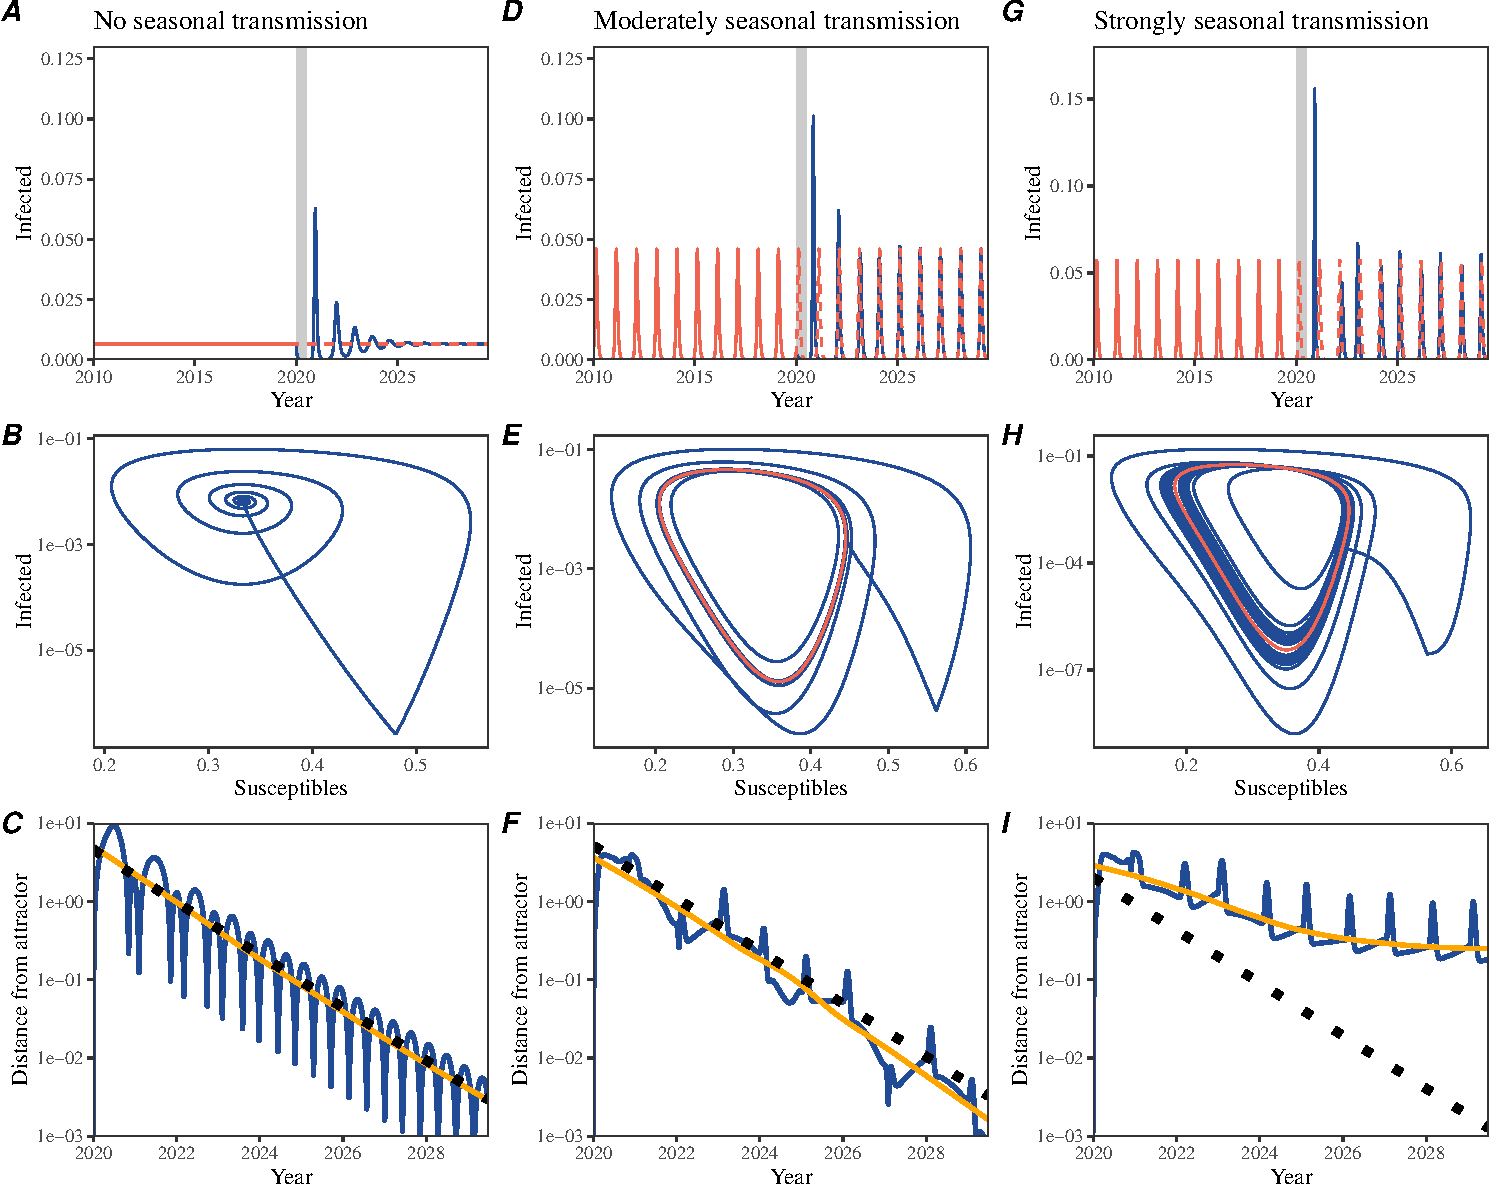
\includegraphics[width=\textwidth]{../figure2/figure2_simple_seas.pdf}
\caption{
\textbf{Impact of seasonal transmission on pathogen resilience.}
(A, D, G) Simulated epidemic trajectories using the SIRS model without seasonal forcing (A), with seasonal forcing of amplitude of 0.2 (D), and with seasonal forcing of amplitude of 0.4 (G).
Red and blue solid lines represent epidemic dynamics before and after interventions are introduced, respectively.
Red dashed lines represent counterfactual epidemic dynamics in the absence of interventions.
Gray regions indicate the duration of interventions.
(B, E, H) Phase plane representation of the corresponding model.
Red and blue solid lines represent epidemic trajectories on an SI phase plane before and after interventions are introduced, respectively.
(C, F, I) Changes in logged distance from the attractor over time.
Blue lines represent the logged distance from the attractor.
Orange lines represent the locally estimated scatterplot smoothing (LOESS) fits to the logged distance from the attractor.
Dotted lines are superimposed as a comparison to have the same slope as the intrinsic resilience of the seasonally unforced system.
}
\end{figure}

\pagebreak

\begin{figure}[!th]
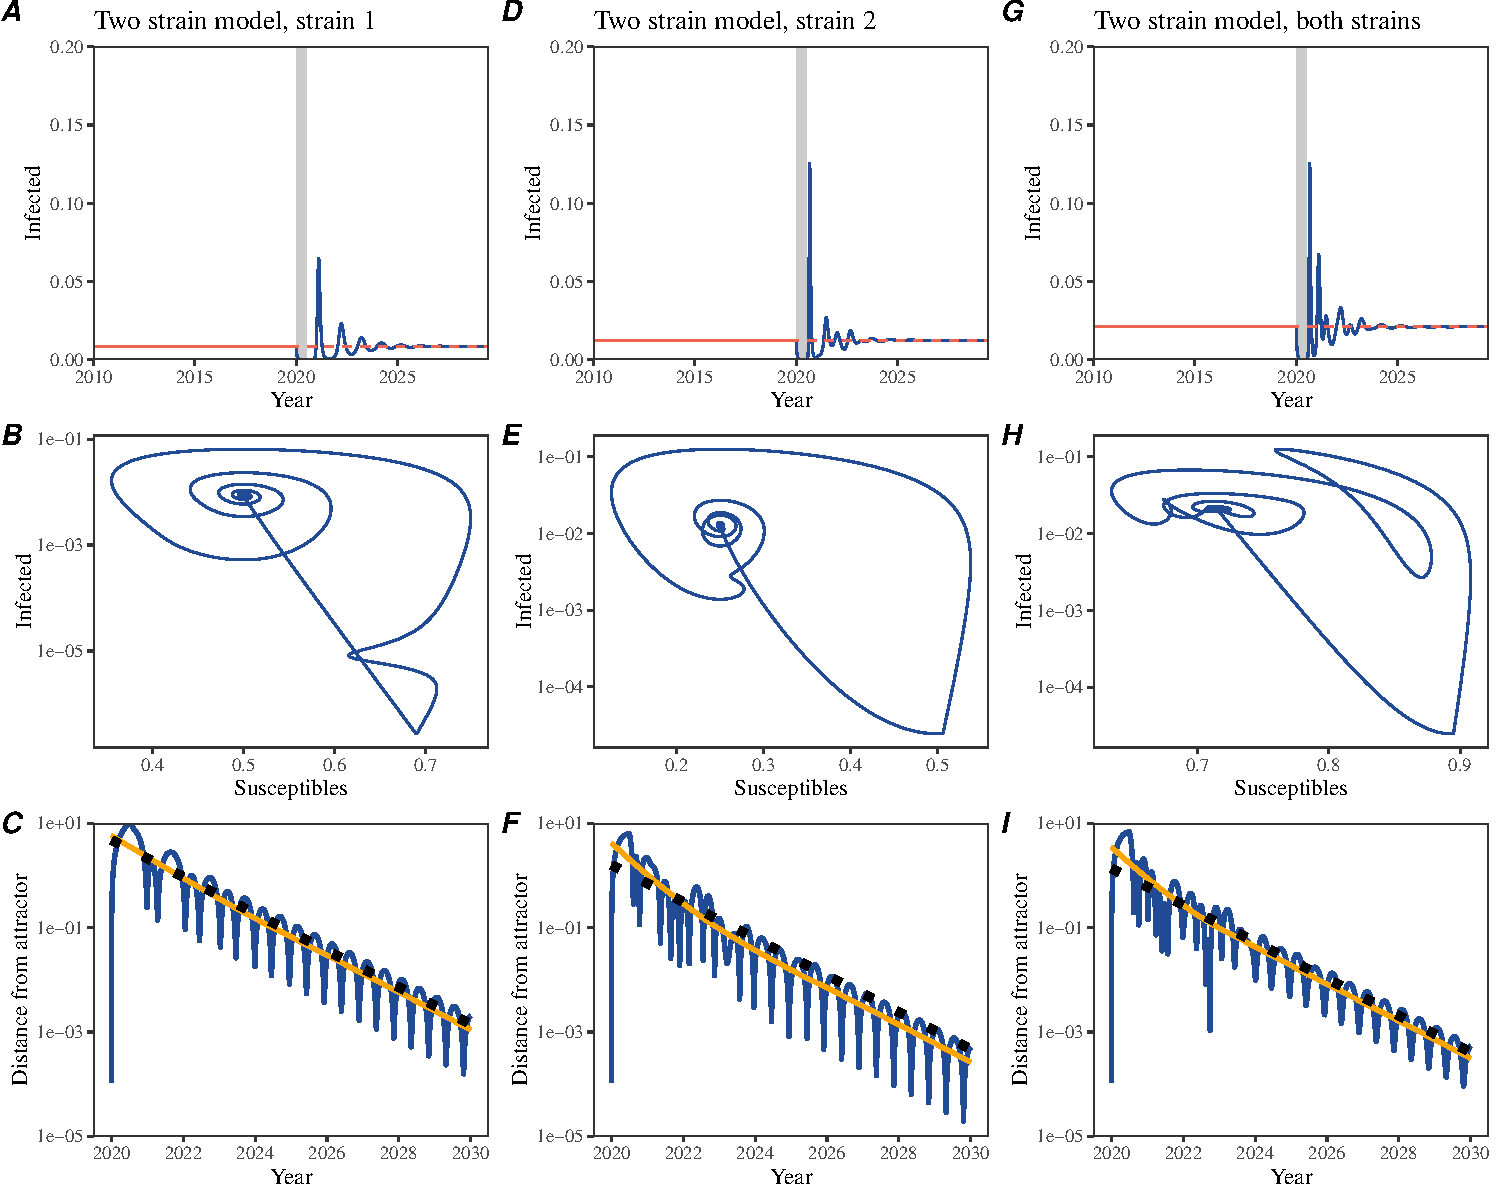
\includegraphics[width=\textwidth]{../figure2/figure2_multi_noseas.pdf}
\caption{
\textbf{Conceptual framework for measuring pathogen resilience following NPIs for a two-strain system without seasonal forcing.}
(A, D, G) Simulated epidemic trajectories using a multi-strain system without seasonal forcing.
Red and blue solid lines represent epidemic dynamics before and after interventions are introduced, respectively.
Red dashed lines represent counterfactual epidemic dynamics in the absence of interventions.
Gray regions indicate the duration of interventions.
(B, E, H) Phase plane representation of the corresponding model.
Blue solid lines represent epidemic trajectories on an SI phase plane before and after interventions are introduced, respectively.
(C, F, I) Changes in logged distance from the attractor over time.
Blue lines represent the logged distance from the attractor.
Orange lines represent the locally estimated scatterplot smoothing (LOESS) fits to the logged distance from the attractor.
Dotted lines are superimposed as a comparison to have the same slope as the intrinsic resilience of the seasonally unforced system.
}
\end{figure}

\pagebreak

\begin{figure}[!th]
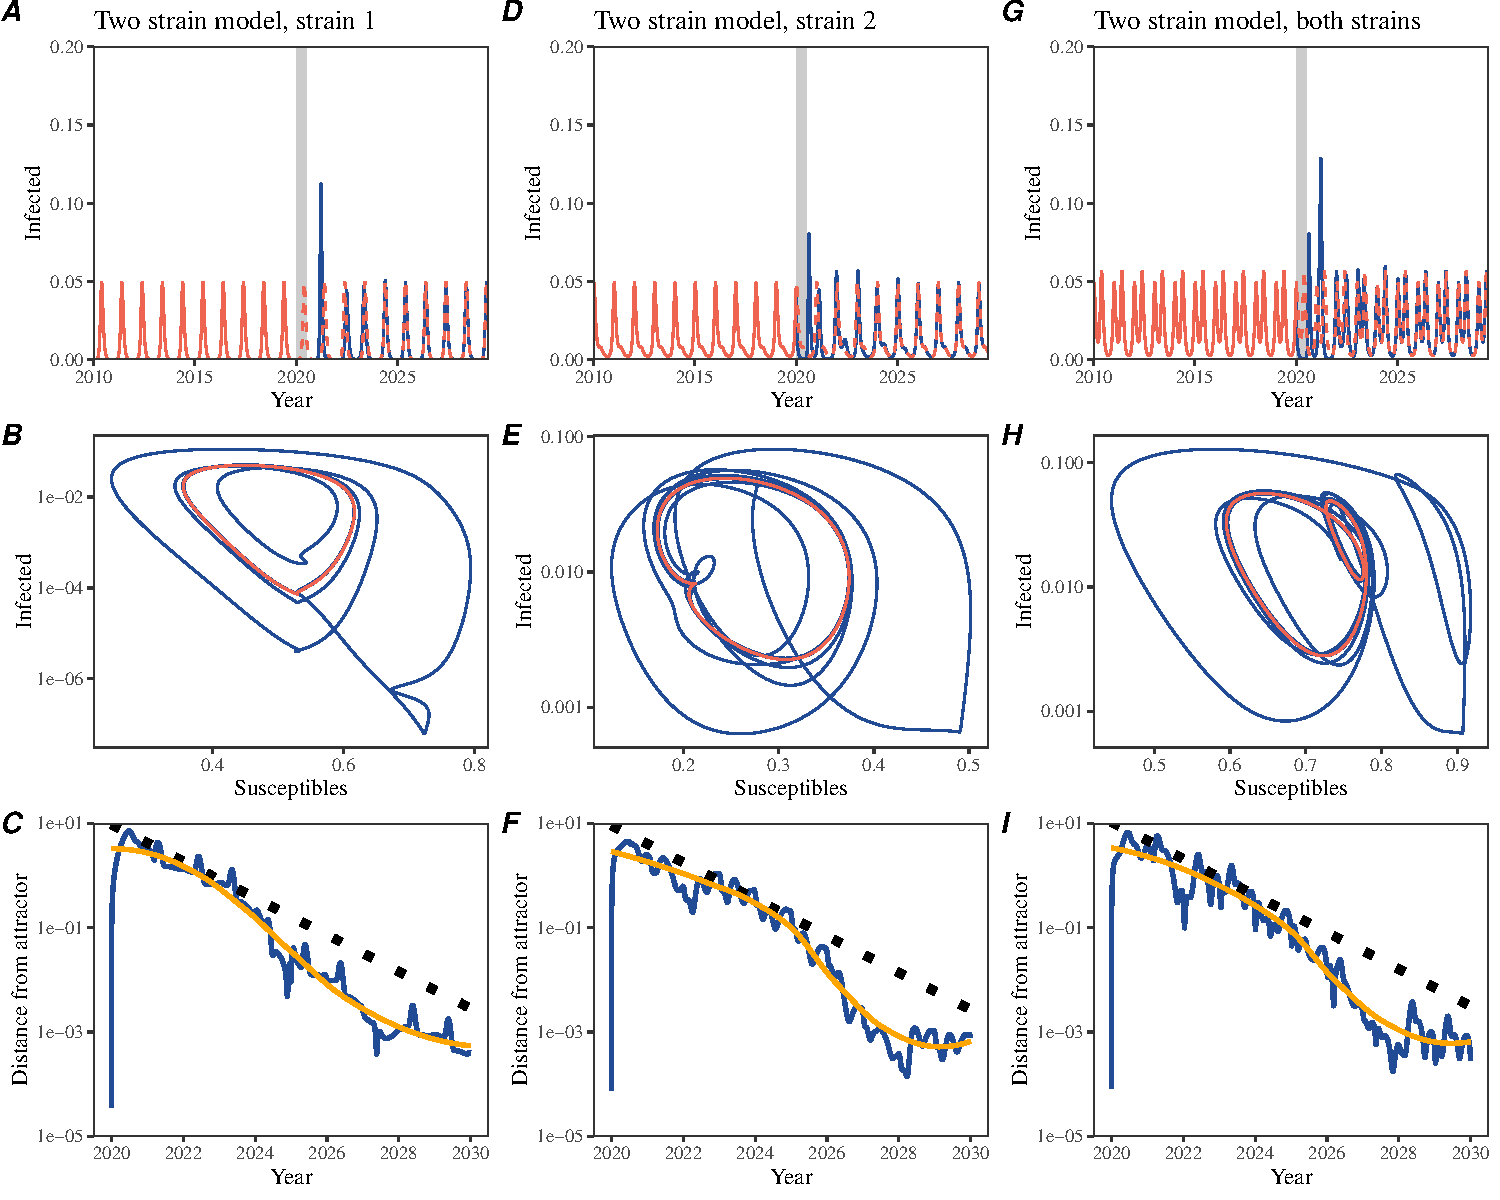
\includegraphics[width=\textwidth]{../figure2/figure2_multi.pdf}
\caption{
\textbf{Conceptual framework for measuring pathogen resilience following NPIs for a multi-strain system with seasonal forcing.}
(A, D, G) Simulated epidemic trajectories using a multi-strain system with seasonal forcing (amplitude of 0.2).
Red and blue solid lines represent epidemic dynamics before and after interventions are introduced, respectively.
Red dashed lines represent counterfactual epidemic dynamics in the absence of interventions.
Gray regions indicate the duration of interventions.
(B, E, H) Phase plane representation of the corresponding model.
Red and blue solid lines represent epidemic trajectories on an SI phase plane before and after interventions are introduced, respectively.
(C, F, I) Changes in logged distance from the attractor over time.
Blue lines represent the logged distance from the attractor.
Orange lines represent the locally estimated scatterplot smoothing (LOESS) fits to the logged distance from the attractor.
Dotted lines are superimposed as a comparison to have the same slope as the intrinsic resilience of the seasonally unforced system.
}
\end{figure}

\pagebreak

\begin{figure}[!th]
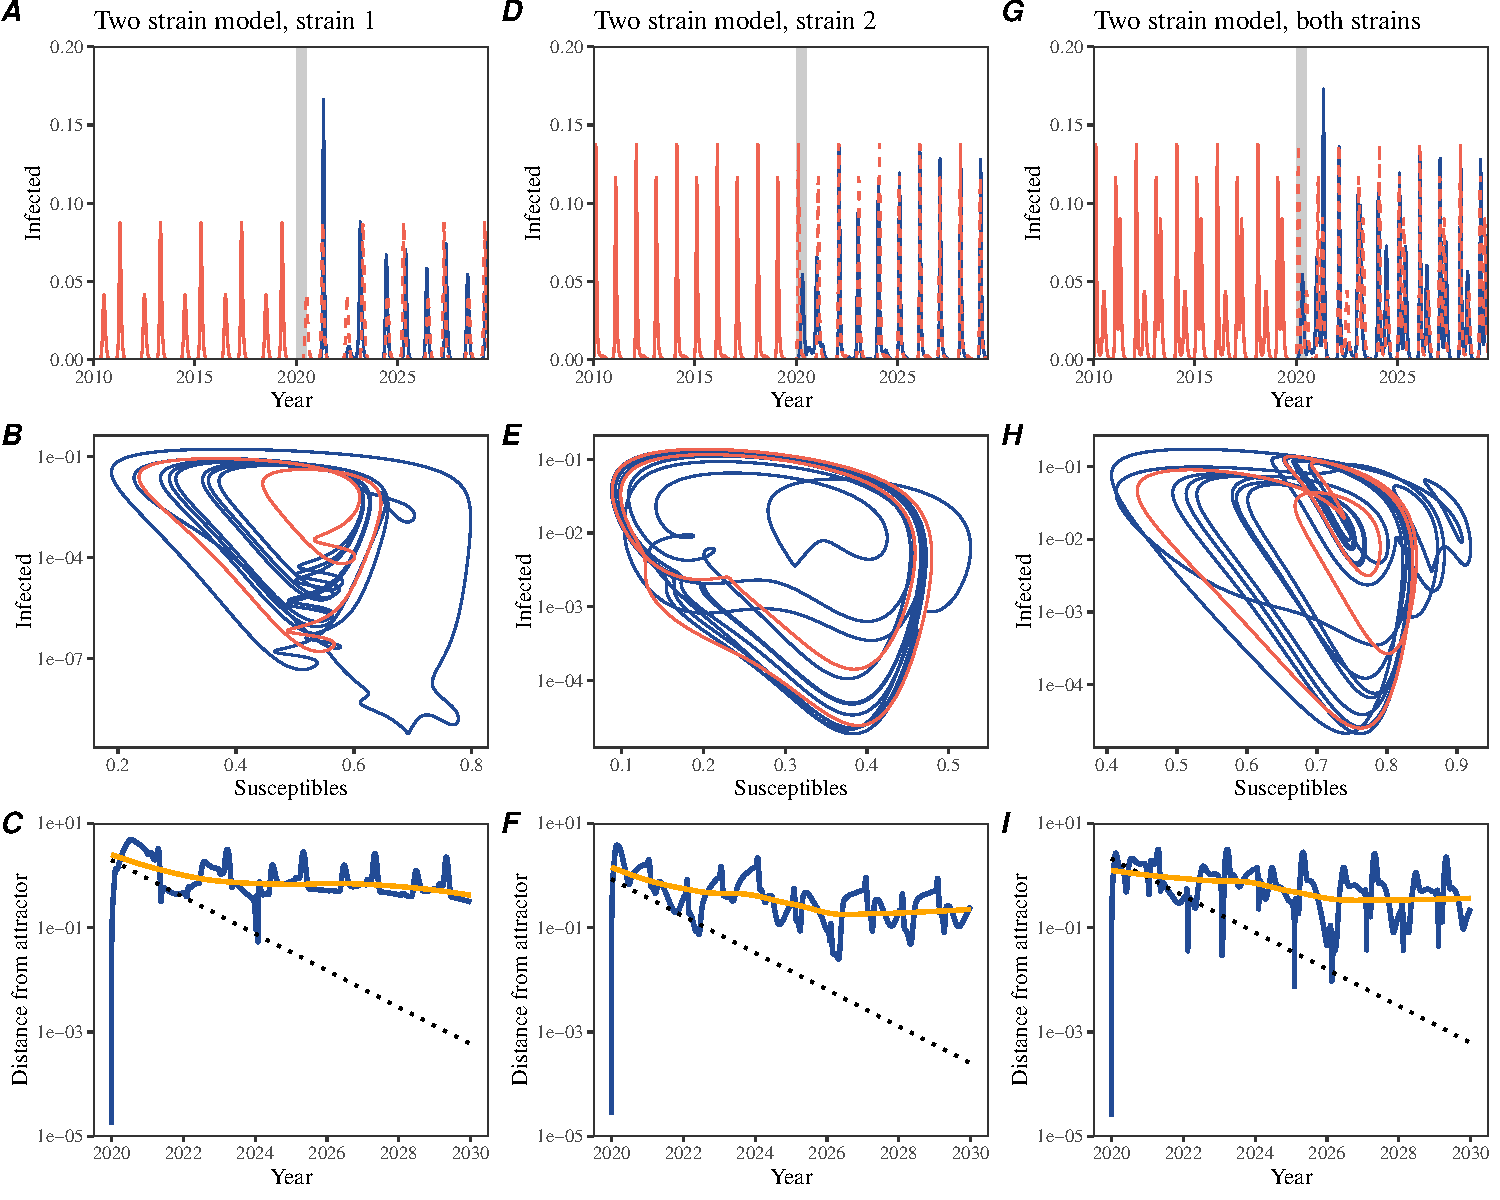
\includegraphics[width=\textwidth]{../figure2/figure2_multi_strong.pdf}
\caption{
\textbf{Conceptual framework for measuring pathogen resilience following NPIs for a multi-strain system with strong seasonal forcing.}
(A, D, G) Simulated epidemic trajectories using a multi-strain system with seasonal forcing (amplitude of 0.4).
Red and blue solid lines represent epidemic dynamics before and after interventions are introduced, respectively.
Red dashed lines represent counterfactual epidemic dynamics in the absence of interventions.
Gray regions indicate the duration of interventions.
(B, E, H) Phase plane representation of the corresponding model.
Red and blue solid lines represent epidemic trajectories on an SI phase plane before and after interventions are introduced, respectively.
(C, F, I) Changes in logged distance from the attractor over time.
Blue lines represent the logged distance from the attractor.
Orange lines represent the locally estimated scatterplot smoothing (LOESS) fits to the logged distance from the attractor.
Dotted lines are superimposed as a comparison to have the same slope as the intrinsic resilience of the seasonally unforced system.
}
\end{figure}

\pagebreak

\begin{figure}[!th]
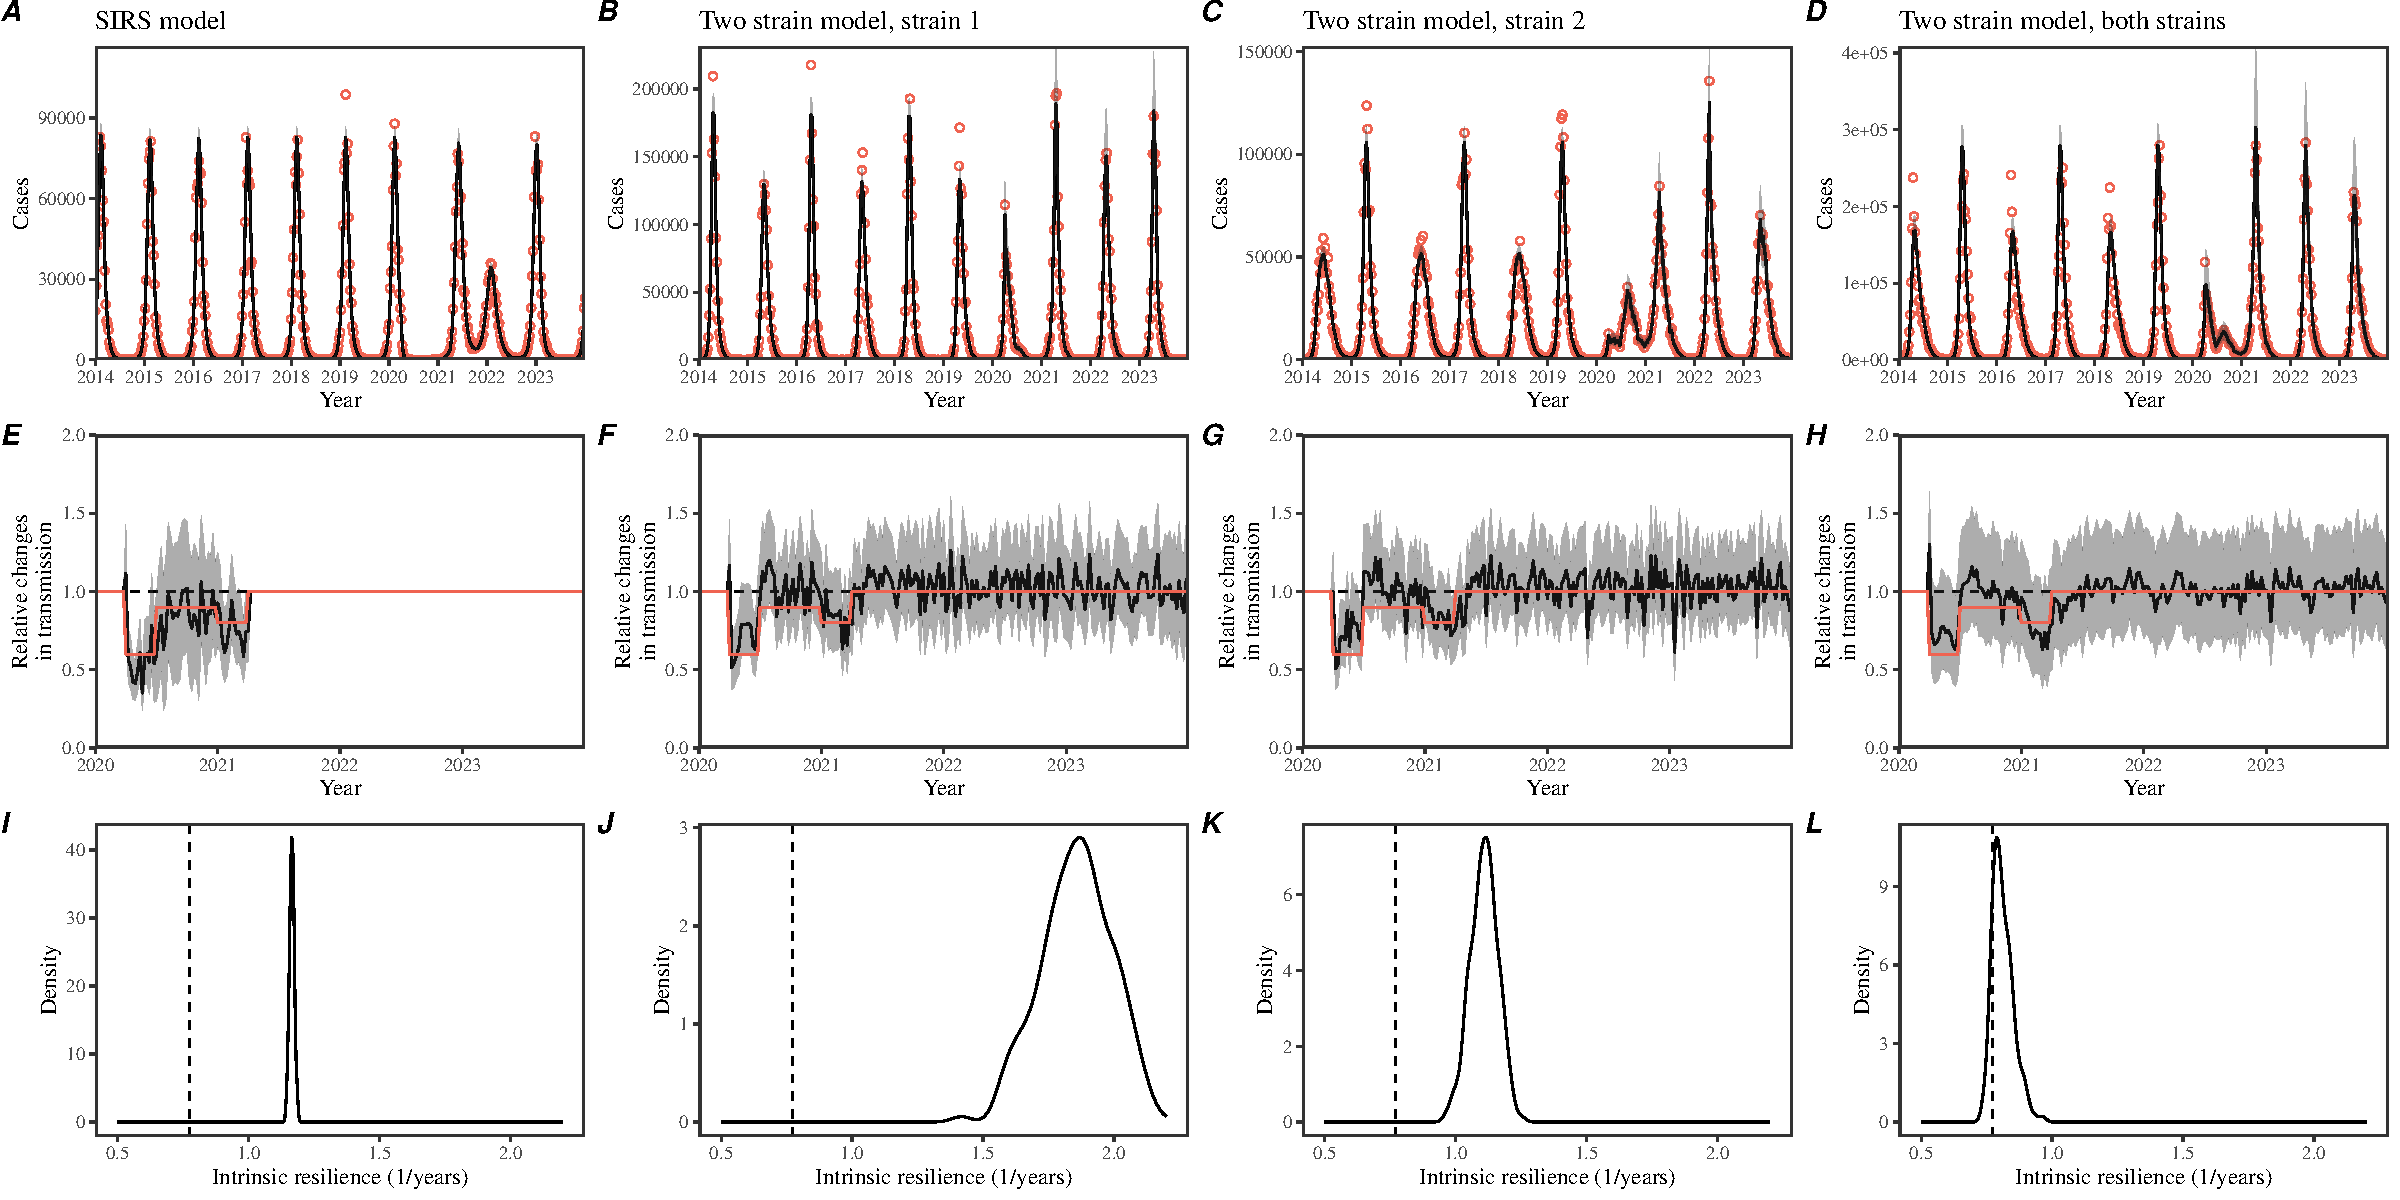
\includegraphics[width=\textwidth]{../figure_fit/figure_fit.pdf}
\caption{
\textbf{Mechanistic model fits to simulated data and inferred intrinsic resilience.}
(A, D, G, J) Simulated case time series from corresponding models (red) and SIRS model fits (black).
(B, E, H, K) Assumed changes in transmission due to pandemic NPIs (red) and estimated changes from the SIRS model (black).
Solid lines and shaded regions represent fitted posterior median and 95\% credible intervals.
(C, F, I, L) True intrinsic resilience of the seasonally unforced system (vertical lines) and the posterior distribution of the inferred intrinsic resilience from the SIRS model (density plots).
}
\end{figure}


\pagebreak

\begin{figure}[!th]
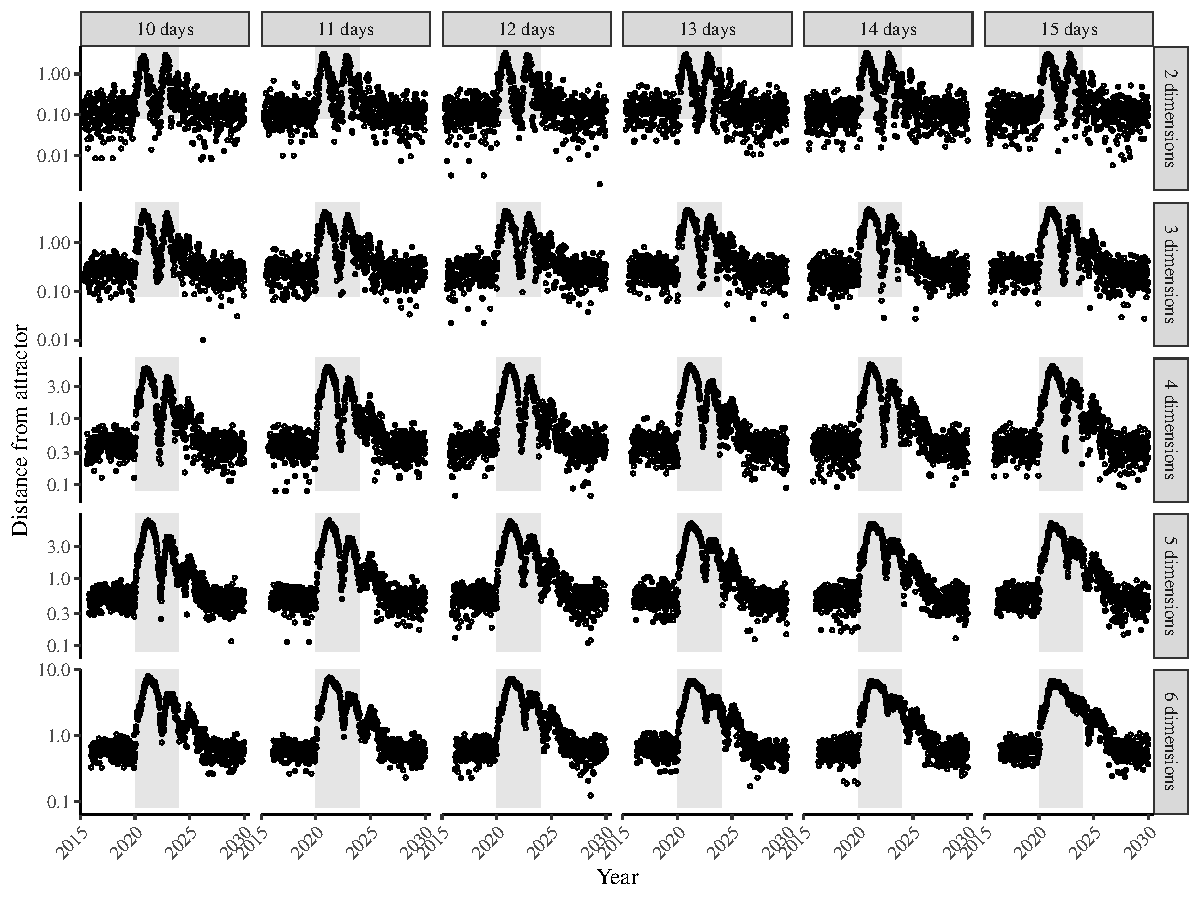
\includegraphics[width=\textwidth]{../figure3/figure3_sens.pdf}
\caption{
\textbf{Sensitivity of the distance from the attractor to choices about emedding lags and dimensions.}
Sensitivity analysis for the distance-from-attractor time series shown in Figure 3E in the main text by varying the embedding lag between 10--15 days and embedding dimensions between 2--6 dimensions.
}
\end{figure}

\pagebreak

\begin{figure}[!th]
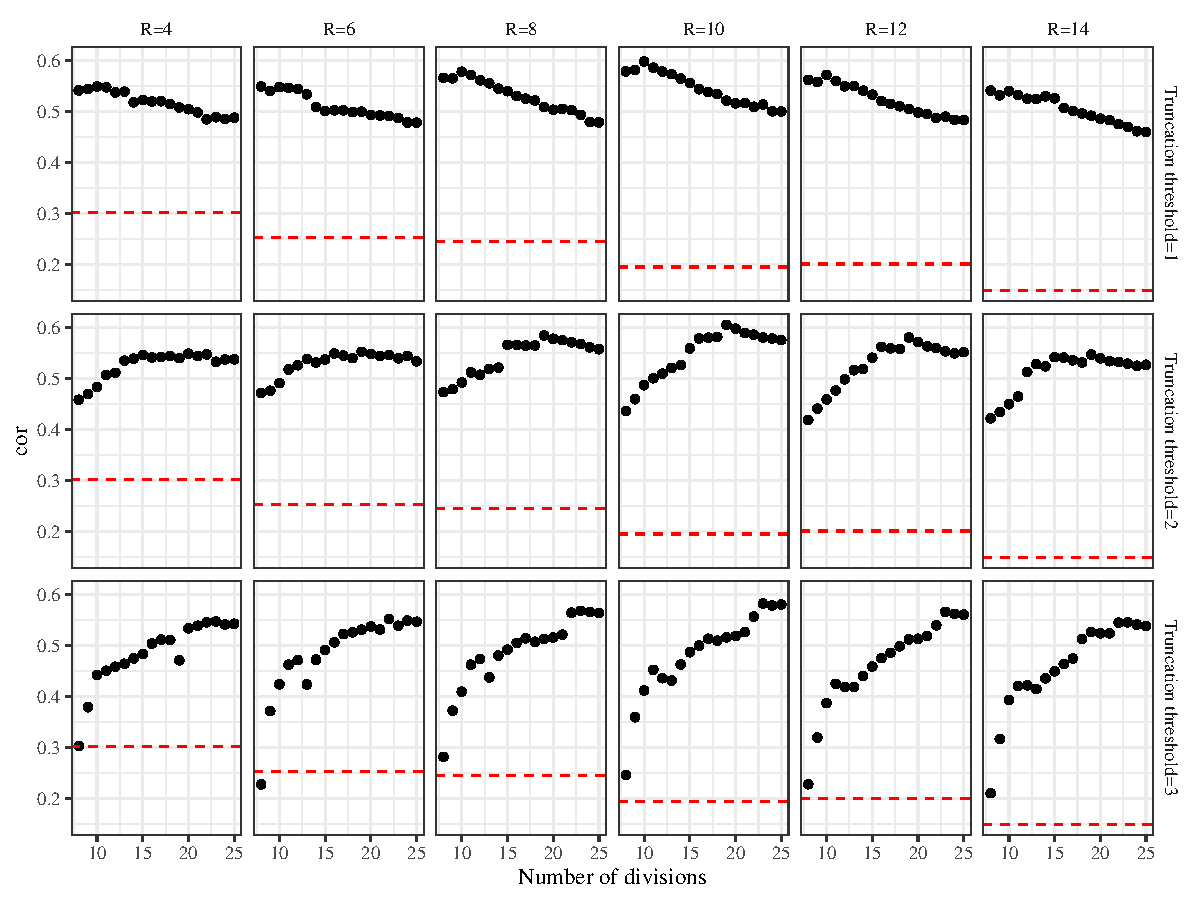
\includegraphics[width=\textwidth]{../figure_analysis_random/figure_analysis_random.pdf}
\caption{
\textbf{Impact of fitting window selection on the estimation of empirical resilience.}
We simulated 500 epidemics of a stochastic SIRS model with randomly drawn parameters and randomly generated intervention impacts.
For each simulation, we reconstructed the empirical attractor based on the approach outlined in Figure 3 and estimate the distance from the attractor.
The naive approach fits a linear regression on a log scale, starting from the maximum distance until the end of the time series.
The window-based approach tries to select an appropriate window by smoothing the distance estimates and finding the time period when the smoothed time series crosses pre-determined threshold, relative to the maximum distance;
then, a linear regression is fitted by using the raw distance within this time period.
}
\end{figure}

\pagebreak

\begin{figure}[!th]
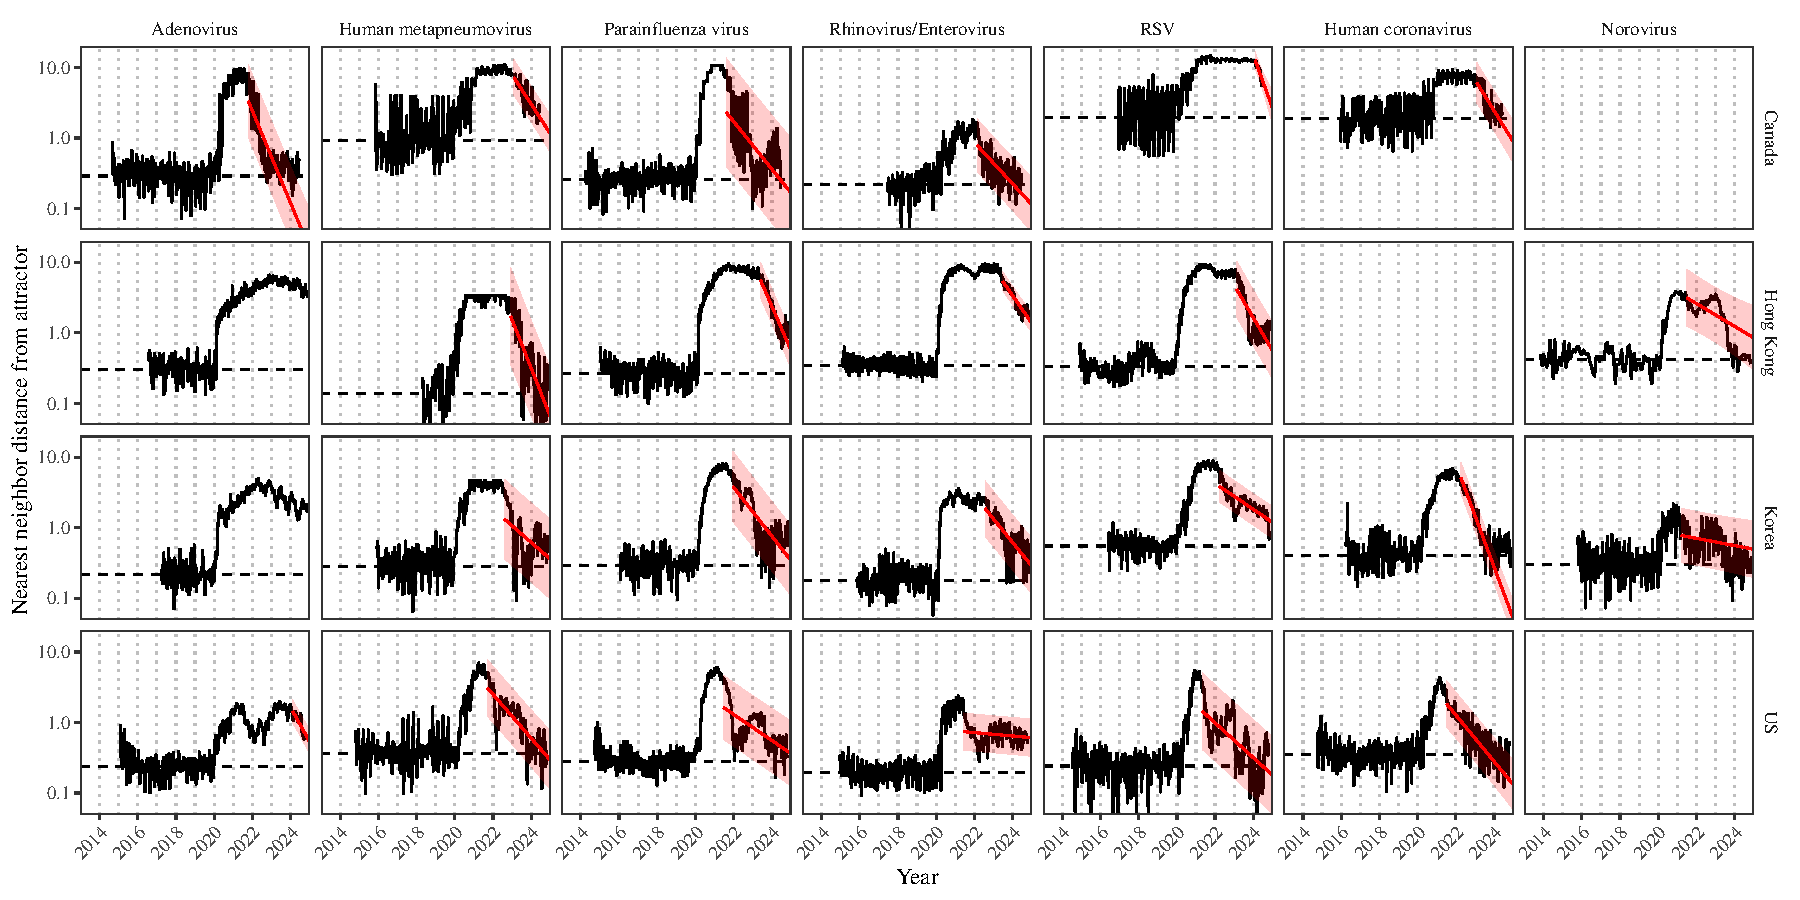
\includegraphics[width=\textwidth]{../figure4/figure4_dist_auto.pdf}
\caption{
\textbf{Estimated time series of distance from the attractor for each pathogen and corresponding linear regression fits using automated window selection criterion across Canada, Hong Kong, Korea, and the US.}
Black lines represent the estimated distance from the attractor.
Red lines and shaded regions represent the linear regression fits and corresponding 95\% confidence intervals.
Dashed lines represent the average of the pre-pandemic nearest neighbor distances.
}
\end{figure}

\pagebreak

\begin{figure}[!th]
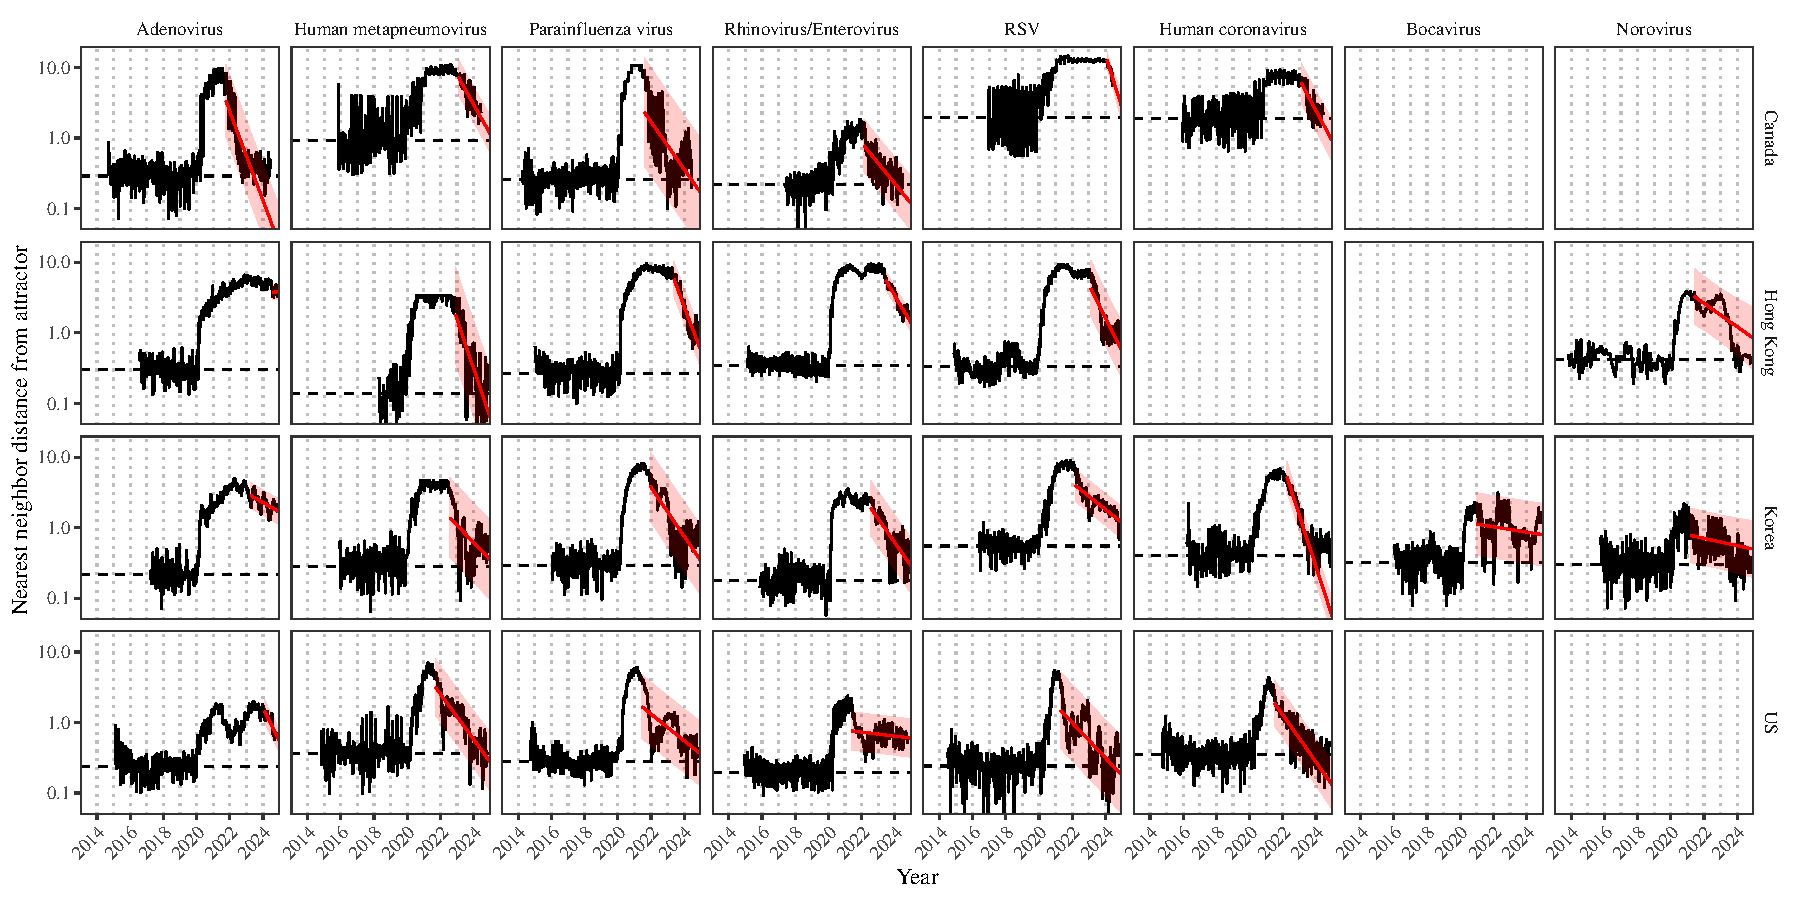
\includegraphics[width=\textwidth]{../figure4/figure4_dist.pdf}
\caption{
\textbf{Estimated time series of distance from the attractor for each pathogen and corresponding linear regression fits across Canada, Hong Kong, Korea, and the US, including ad-hoc regression window selection.}
We used ad-hoc regression windows for norovirus in Hong Kong and Korea and Rhinovirus/Enterovirus in the US.
Black lines represent the estimated distance from the attractor.
Red lines and shaded regions represent the linear regression fits and corresponding 95\% confidence intervals.
Dashed lines represent the average of the pre-pandemic nearest neighbor distances.
}
\end{figure}

\pagebreak

\begin{figure}[!th]
\begin{center}
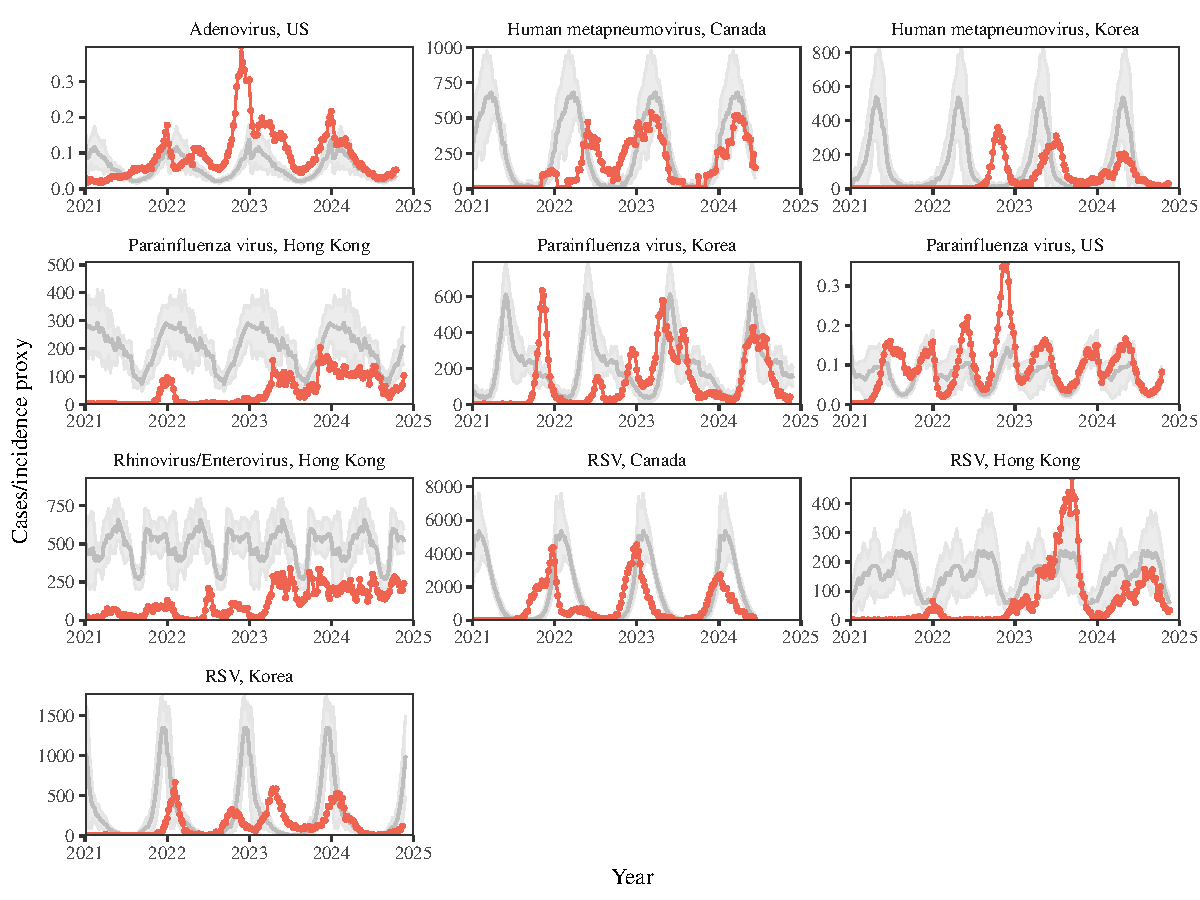
\includegraphics[width=\textwidth]{../figure4/figure4_noreturn.pdf}
\caption{
\textbf{Observed dynamics for pathogen that are predicted to return after the end of 2024.}
Red points and lines represent data before 2020.
Gray lines and shaded regions represent the mean seasonal patterns and corresponding 95\% confidence intervals around the mean, previously shown in Figure 1.
}
\end{center}
\end{figure}


\pagebreak

\begin{figure}[!th]
\begin{center}
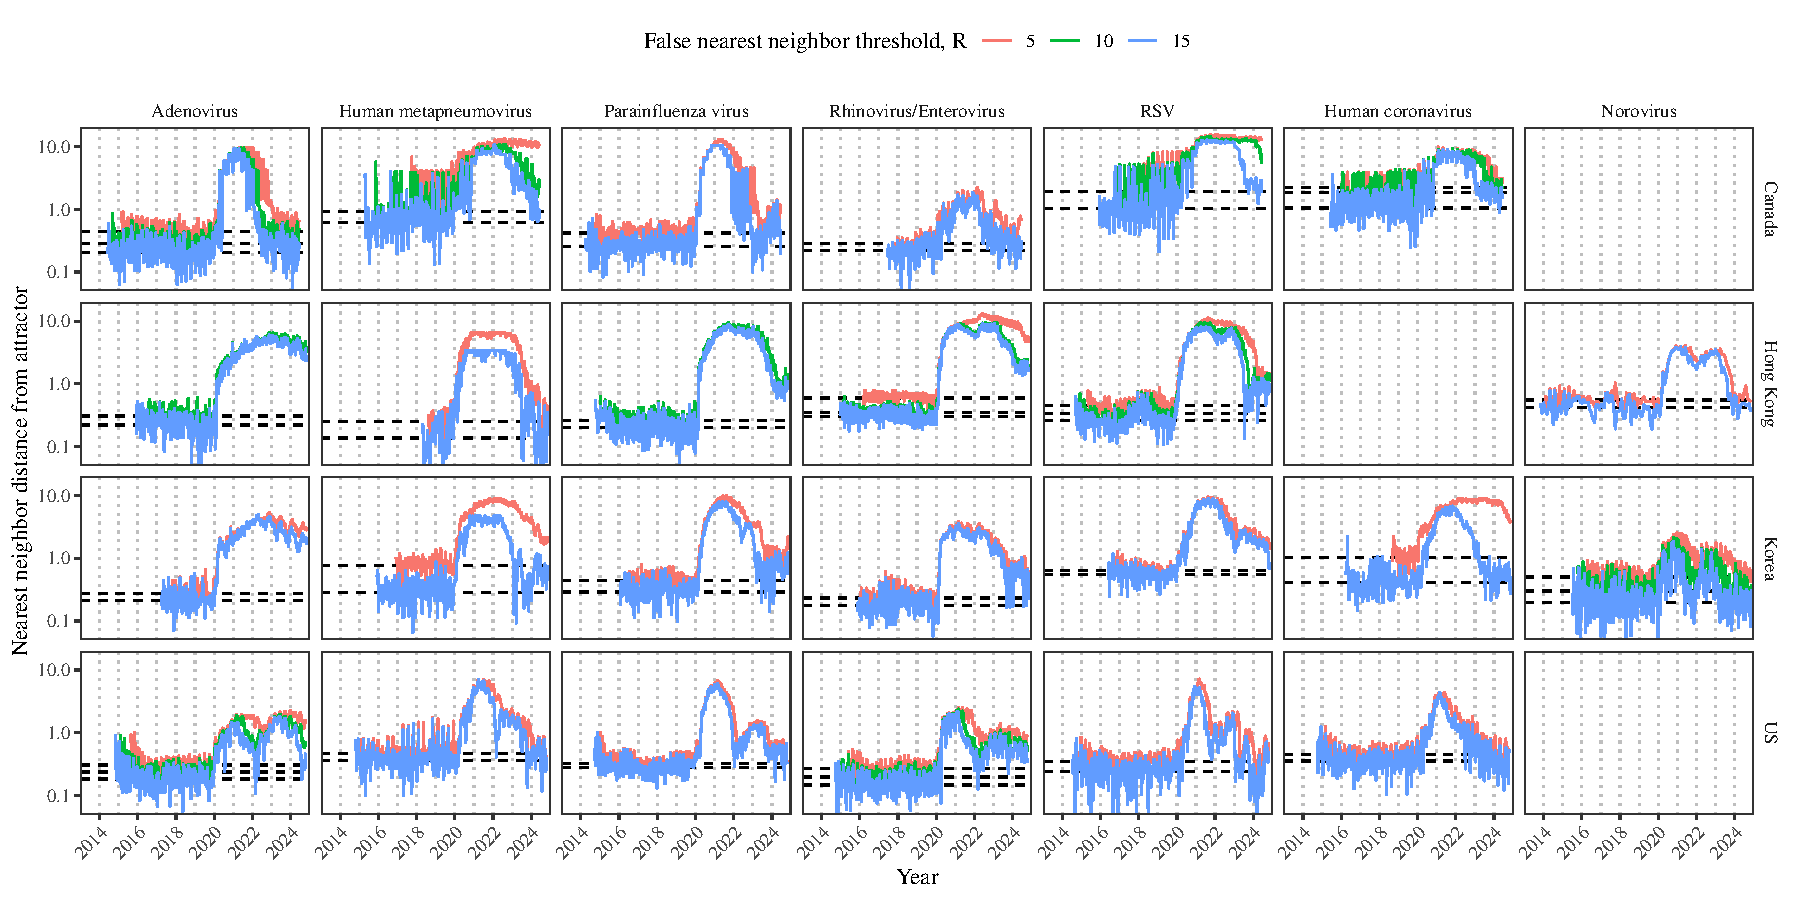
\includegraphics[width=\textwidth]{../figure4_R/figure4_dist_R.pdf}
\caption{
\textbf{Estimated time series of distance from the attractor for each pathogen across different choices about false nearest neighbor threshold values.}
Using higher threshold values for the false nearest neighbor approach gives lower embedding dimensions.
Colored lines represent the estimated distance from the attractor for different threshold values.
}
\end{center}
\end{figure}

\pagebreak

\begin{figure}[!th]
\begin{center}
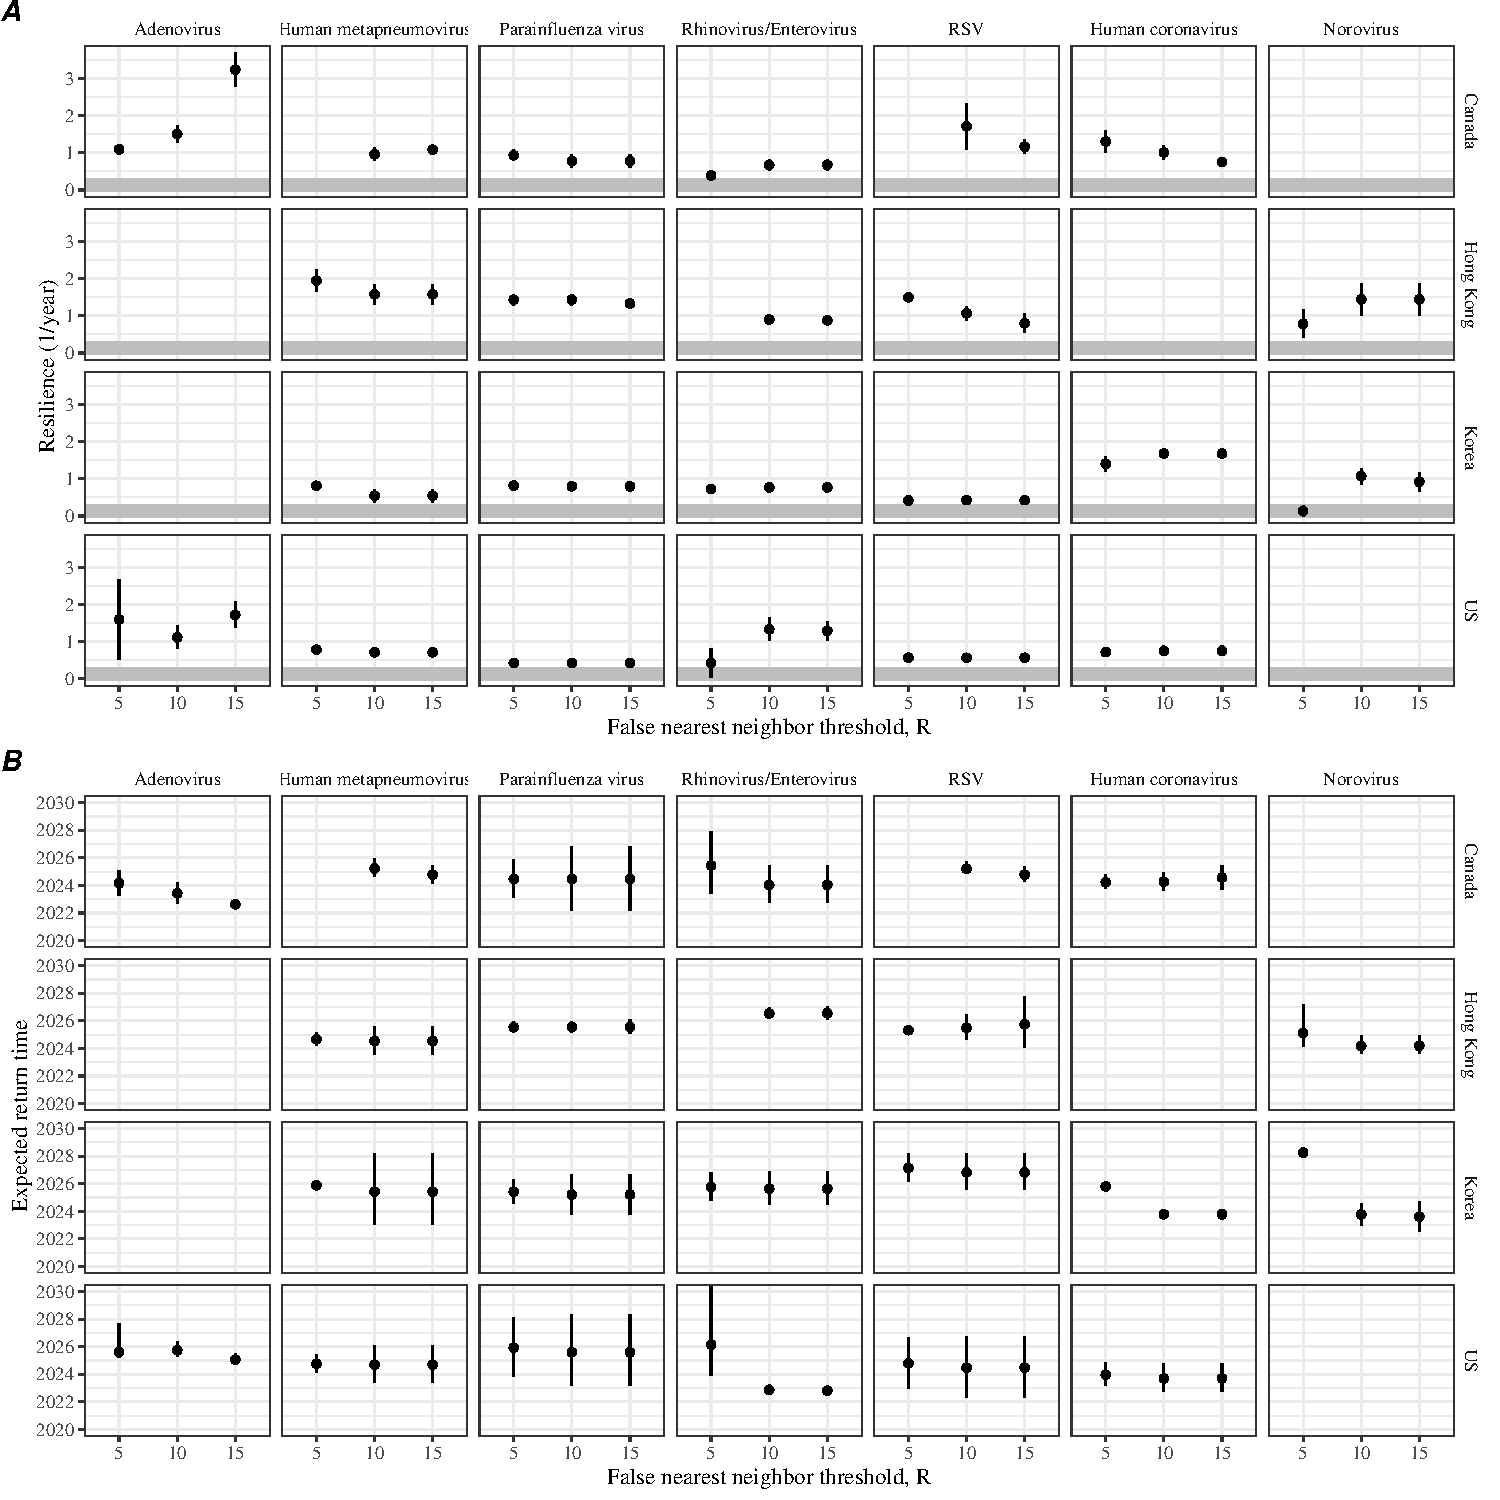
\includegraphics[width=0.9\textwidth]{../figure4_R/figure4_R.pdf}
\caption{
\textbf{Summary of resilience estimates and predictions for return time across different choices about false nearest neighbor threshold values.}
The automated window selection method was used for all scenarios to estimate pathogen resilience, except for norovirus in Hong Kong and Korea and Rhinovirus/Enterovirus in the US.
We used the same ad-hoc regression windows for norovirus in Hong Kong and Korea and Rhinovirus/Enterovirus in the US as we did in the main analysis.
(A) Estimated pathogen resilience.
The gray horizontal line represents the intrinsic resilience of pre-vaccination measles dynamics.
(B) Predicted timing of when each pathogen will return to their pre-pandemic cycles.
The dashed line in panel B indicates the end of 2024 (current observation time).
Error bars represent 95\% confidence intervals.
}
\end{center}
\end{figure}

\pagebreak


\begin{figure}[!th]
\begin{center}
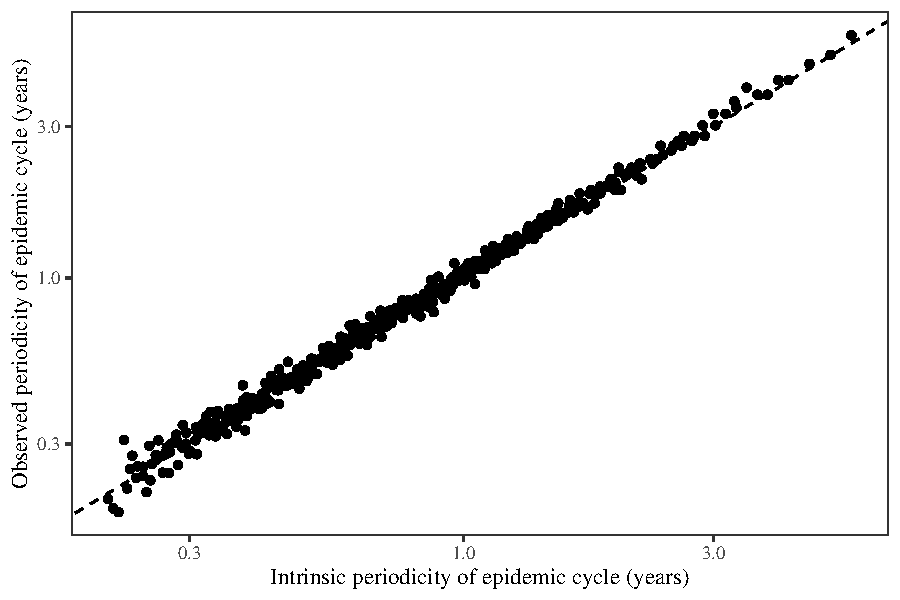
\includegraphics[width=\textwidth]{../figure6/figure_persistence_noise_period.pdf}
\caption{
\textbf{Comparison between the observed and predicted periodicity of the epidemic cycle of the seasonally unforced SIRS model.}
The observed periodicity of the epidemic corresponds to the periodicity at which maximum spectral density occurs.
The predicted periodicity of the epidemic corresponds to $2 \pi/\mathrm{Im}(\lambda)$, where $\mathrm{Im}(\lambda)$ is the imaginary part of the eigenvalue.
}
\end{center}
\end{figure}

\pagebreak

\begin{figure}[!th]
\begin{center}
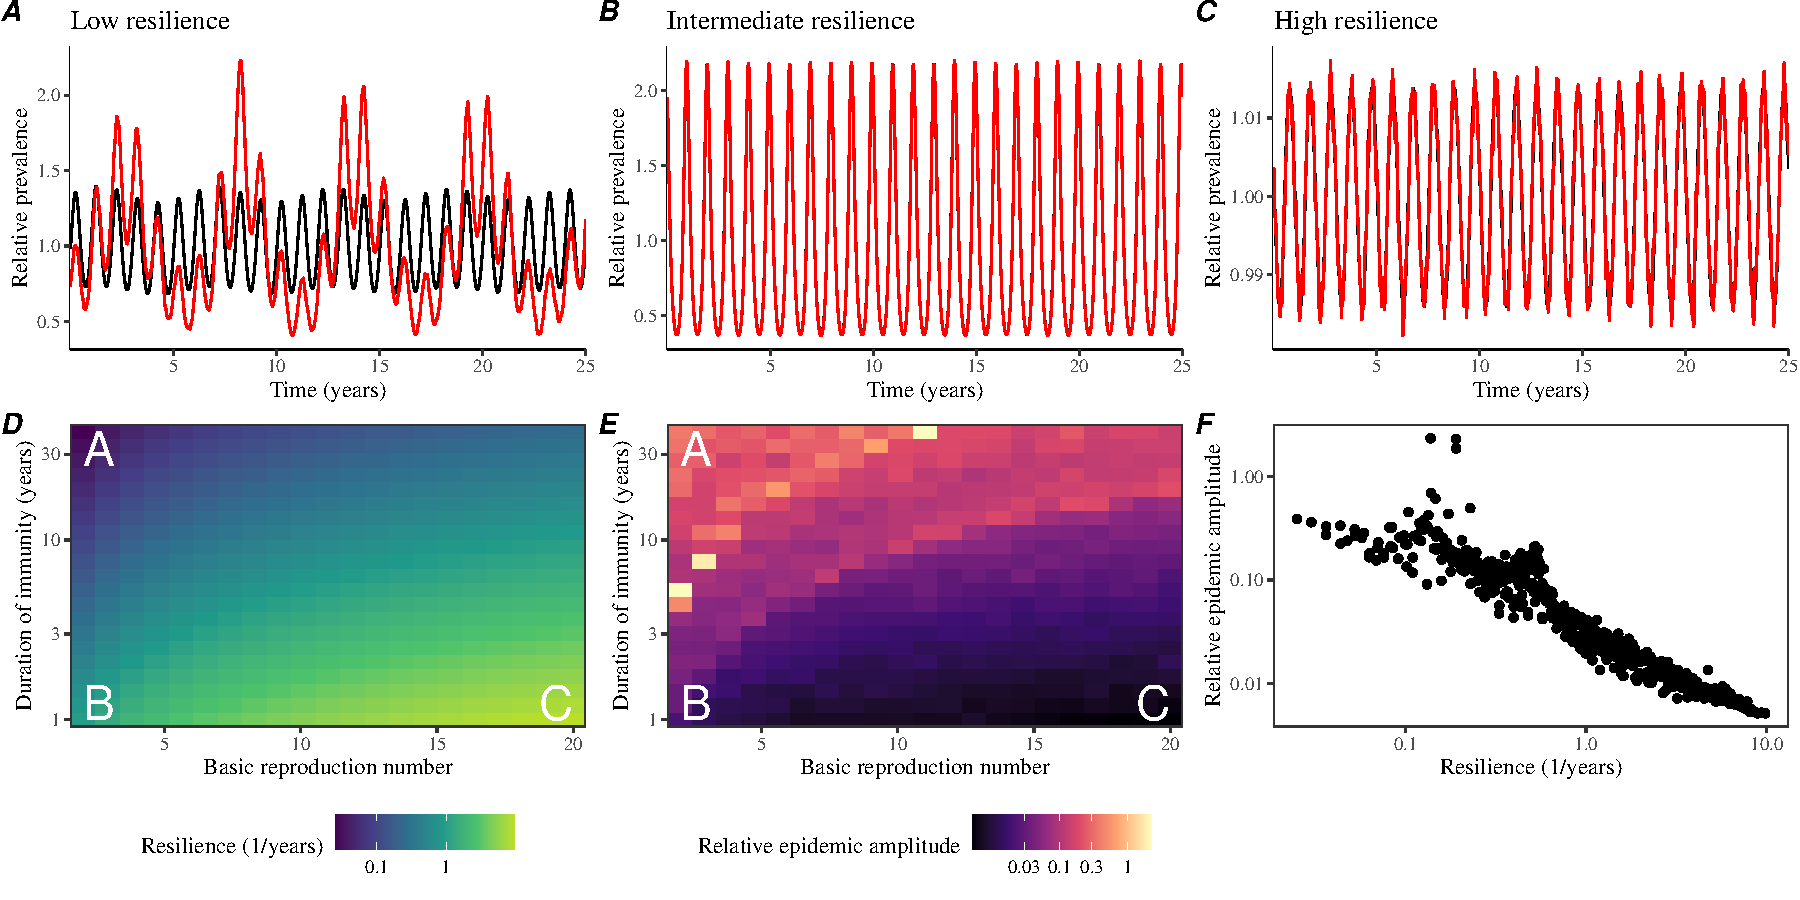
\includegraphics[width=\textwidth]{../figure6/figure_persistence_noise_cycle.pdf}
\caption{
\textbf{Linking resilience of a host-pathogen system to its sensitivity to stochastic perturbations for the seasonally forced SIRS model.}
(A--C) Epidemic trajectories of a stochastic SIRS model across three different resilience values: low, intermediate, and high.
The relative prevalence was calculated by dividing infection prevalence by its mean value.
(D) The heat map represents the intrinsic resilience of the seasonally unforced system as a function of the basic reproduction number $\mathcal R_0$ and the duration of immunity.
(E) The heat map represents the relative epidemic amplitude as a function of the basic reproduction number $\mathcal R_0$ and the duration of immunity.
To calculate the relative epidemic amplitude, we first take the relative difference in infection prevalence between stochastic and deterministic trajectories: $\epsilon = (\tsub{I}{stoch}-\tsub{I}{det})/\tsub{I}{det}$. 
Then, we calculate the difference between maximum and minimum of the relative difference and divide by half: $(\max \epsilon - \min \epsilon)/2$.
(F) The relationship between pathogen resilience and relative epidemic amplitude.
}
\end{center}
\end{figure}


\pagebreak

\bibliography{return-time.bib}

\end{document}
